% !TeX program = latexmk
% !TeX encoding = UTF-8
% =====================================================================
%  TESIS DE GRADO – CARRERA DE INGENIERÍA CIVIL – UATF
%  Compilar desde esta carpeta con:   latexmk
%  (pdflatex + biber; configuración en .latexmkrc; PDF en build/tesis.pdf)
% =====================================================================
\documentclass[12pt,letterpaper,oneside]{report}
% =====================================================================
%  PREÁMBULO DE LA TESIS: paquetes y formato
%  Ajuste aquí márgenes, letra e interlineado si el Reglamento de
%  Graduación de la Carrera de Ingeniería Civil (UATF) exige otros valores.
% =====================================================================

% --- Idioma, codificación y letra ------------------------------------
\usepackage[T1]{fontenc}
\usepackage[spanish,es-tabla,es-noshorthands,es-lcroman]{babel}
\usepackage{amsmath}
\usepackage{newtxtext,newtxmath}      % letra tipo Times New Roman
\renewcommand{\ttdefault}{lmtt}       % monoespaciada (rutas y DOI): Latin Modern
% El mapa de fuentes de MiKTeX de este equipo no registra newtx (MiKTeX
% indica "User/administrator updates are out-of-sync"); se carga aquí:
\pdfmapfile{+newtx.map}
\pdfmapfile{+qtm.map}   % TeX Gyre Termes (símbolos TS1 de newtxtext)
\pdfmapfile{+qhv.map}   % TeX Gyre Heros (sans)
\usepackage[protrusion=true,expansion=false]{microtype}
\usepackage[autostyle]{csquotes}

% --- Página: tamaño carta, márgenes e interlineado --------------------
\usepackage[letterpaper,top=2.5cm,bottom=2.5cm,left=3cm,right=2.5cm,
            headheight=15pt,footskip=1.2cm]{geometry}
\usepackage{setspace}
\onehalfspacing                         % interlineado 1,5
\setlength{\parindent}{0pt}
\setlength{\parskip}{6pt plus 2pt minus 1pt}

% --- Colores, cajas y utilidades --------------------------------------
\usepackage[dvipsnames,table]{xcolor}
\usepackage{etoolbox}
\usepackage[inline]{enumitem}
\setlist{itemsep=2pt,topsep=4pt,parsep=0pt,leftmargin=*}

% --- Títulos de capítulos y secciones ---------------------------------
\usepackage{titlesec}
\titleformat{\chapter}[display]
  {\normalfont\large\bfseries\centering}
  {\MakeUppercase{\chaptertitlename}\ \thechapter}{6pt}{\MakeUppercase}
\titleformat{name=\chapter,numberless}[block]
  {\normalfont\large\bfseries\centering}{}{0pt}{\MakeUppercase}
\titlespacing*{\chapter}{0pt}{0pt}{18pt}
\titleformat{\section}{\normalfont\normalsize\bfseries}{\thesection.}{0.6em}{}
\titleformat{\subsection}{\normalfont\normalsize\bfseries}{\thesubsection.}{0.6em}{}
\titleformat{\subsubsection}{\normalfont\normalsize\bfseries\itshape}{\thesubsubsection.}{0.6em}{}
\titlespacing*{\section}{0pt}{12pt}{4pt}
\titlespacing*{\subsection}{0pt}{10pt}{3pt}
\titlespacing*{\subsubsection}{0pt}{8pt}{2pt}
\setcounter{secnumdepth}{3}
\setcounter{tocdepth}{2}

% --- Nombres en español ------------------------------------------------
\addto\captionsspanish{%
  \renewcommand{\contentsname}{Índice general}%
  \renewcommand{\listtablename}{Índice de tablas}%
  \renewcommand{\listfigurename}{Índice de figuras}%
  \renewcommand{\appendixname}{Anexo}%
  \renewcommand{\bibname}{Bibliografía}%
}

% --- Índices (tabla de contenido) -------------------------------------
\usepackage{tocloft}
\renewcommand{\cftchapfont}{\bfseries}
\renewcommand{\cftchappagefont}{\bfseries}
\renewcommand{\cftchapleader}{\cftdotfill{\cftdotsep}}
\renewcommand{\cftchappresnum}{\chaptername\ }
\renewcommand{\cftchapaftersnum}{.}
\setlength{\cftchapnumwidth}{6.4em}
\setlength{\cftbeforechapskip}{6pt}
\renewcommand{\cfttabpresnum}{Tabla\ }
\renewcommand{\cftfigpresnum}{Figura\ }
\renewcommand{\cfttabaftersnum}{.}
\renewcommand{\cftfigaftersnum}{.}
\setlength{\cfttabnumwidth}{5.2em}
\setlength{\cftfignumwidth}{5.6em}
\setlength{\cfttabindent}{0pt}
\setlength{\cftfigindent}{0pt}

% --- Tablas ------------------------------------------------------------
\usepackage{array,booktabs,tabularx,longtable,multirow,makecell}
\renewcommand{\arraystretch}{1.15}
\newcolumntype{L}{>{\raggedright\arraybackslash}X}
\newcolumntype{C}{>{\centering\arraybackslash}X}
\newcolumntype{P}[1]{>{\raggedright\arraybackslash}p{#1}}
\newcolumntype{Q}[1]{>{\centering\arraybackslash}p{#1}}
\AtBeginEnvironment{table}{\small\setstretch{1}}
\AtBeginEnvironment{figure}{\setstretch{1}}

% --- Leyendas de tablas y figuras (estilo APA 7) -----------------------
%     Número en negrita y título en cursiva en la línea siguiente.
\usepackage{caption}
\captionsetup{font={small,stretch=1},labelfont=bf,textfont=it,
              labelsep=newline,justification=raggedright,
              singlelinecheck=false,skip=4pt}
\counterwithout{table}{chapter}         % Tabla 1, 2, 3...
\counterwithout{figure}{chapter}        % Figura 1, 2, 3...
\counterwithout{equation}{chapter}      % (1), (2), (3)...
% Nota debajo de una tabla o figura: \nota{Elaborado con base en ...}
\newcommand{\nota}[1]{\par\vspace{2pt}{\small\setstretch{1}\textit{Nota.} #1\par}}

% --- Figuras, planos y diagramas -----------------------------------------
\usepackage{graphicx}
\graphicspath{{figuras/}}
\usepackage{float}
\usepackage{pdflscape}
\usepackage{pdfpages}
\usepackage{tikz}
\usetikzlibrary{arrows.meta,positioning,babel}

% --- Unidades y números (coma decimal, punto de miles) ------------------
\usepackage{siunitx}
\sisetup{output-decimal-marker={,},group-separator={.},
         group-minimum-digits=4,per-mode=symbol}
\newcommand{\mdos}{m\textsuperscript{2}}    % metro cuadrado
\newcommand{\mtres}{m\textsuperscript{3}}   % metro cúbico

% --- Encabezado y pie de página --------------------------------------
\usepackage{fancyhdr}
\fancypagestyle{tesis}{\fancyhf{}\fancyfoot[C]{\thepage}%
  \renewcommand{\headrulewidth}{0pt}}
\fancypagestyle{plain}{\fancyhf{}\fancyfoot[C]{\thepage}%
  \renewcommand{\headrulewidth}{0pt}}
\pagestyle{tesis}

% --- Marcas de borrador -------------------------------------------------
%  \pendiente{...} : texto o dato que falta completar (rojo).
%  \guia{...}      : instrucciones para redactar una sección (recuadro gris).
%  Ambas desaparecen al poner \borradorfalse en tesis.tex.
\newif\ifborrador
\newcommand{\pendiente}[1]{\ifborrador{\color{BrickRed}\textbf{[Pendiente:} #1\textbf{]}}\fi}
\newcommand{\guia}[1]{\ifborrador\par\noindent
  \fcolorbox{gray!60}{gray!8}{\parbox{\dimexpr\linewidth-2\fboxsep-2\fboxrule\relax}{%
  \small\setstretch{1}\textbf{Guía de desarrollo.} #1}}\par\fi}

% --- Ruta a los datos de obra del repositorio -----------------------------
\newcommand{\datos}{../03_Datos_Obra_Edificio_Posgrado}

% --- Bibliografía APA 7.ª edición -----------------------------------------
\usepackage[style=apa,backend=biber]{biblatex}
\addbibresource{bibliografia.bib}

% --- Hipervínculos (cargar al final) --------------------------------------
\usepackage[hidelinks,bookmarksnumbered]{hyperref}


% ---- Datos generales (se usan en la carátula y en las propiedades del PDF)
\newcommand{\titulotesis}{DISEÑO DE UN SISTEMA DE GESTIÓN DE LA CALIDAD BASADO EN LA NORMA ISO~9001 PARA REDUCIR COSTOS MEDIANTE EL CONTROL DE MATERIALES EN LOSAS ALIVIANADAS CON VIGUETAS PRETENSADAS DEL EDIFICIO DE POSGRADO DE LA UNIVERSIDAD AUTÓNOMA TOMÁS FRÍAS, POTOSÍ}
\newcommand{\postulante}{[Nombres y apellidos del postulante]}
\newcommand{\tutor}{Ing.\ [Nombres y apellidos del tutor]}
\newcommand{\lugar}{POTOSÍ -- BOLIVIA}
\newcommand{\anio}{2026}

\hypersetup{pdftitle={Diseño de un Sistema de Gestión de la Calidad para reducir costos mediante el control de materiales en losas alivianadas - Edificio de Posgrado UATF},
            pdfsubject={Tesis de grado - Ingeniería Civil - UATF}}

% ---- Modo borrador: muestra guías y pendientes.
%      Para la versión final cambie a \borradorfalse
\borradortrue

\begin{document}

% ---------------- Carátula y páginas preliminares (numeración romana)
% =====================================================================
%  CARÁTULA  (verificar el formato exacto en el Reglamento de Graduación)
% =====================================================================
\begin{titlepage}
\centering
\setstretch{1.2}
{\large\bfseries UNIVERSIDAD AUTÓNOMA «TOMÁS FRÍAS»\par}
{\large\bfseries FACULTAD DE INGENIERÍA\par}
{\large\bfseries CARRERA DE INGENIERÍA CIVIL\par}
\vspace{1.4cm}
% Para colocar el escudo: guarde la imagen en figuras/escudo_uatf.png
% y reemplace la línea \pendiente por:
% \includegraphics[width=3.5cm]{escudo_uatf}
\pendiente{insertar el escudo de la UATF}\par
\vspace{1.4cm}
{\large\bfseries TESIS DE GRADO\par}
\vspace{1.0cm}
{\bfseries\titulotesis\par}
\vspace{1.2cm}
{Trabajo de graduación en la modalidad de Tesis, presentado para optar al grado académico de Licenciatura en Ingeniería Civil\par}
\vfill
\begin{tabular}{@{}r@{\hspace{0.6em}}l@{}}
\textbf{Postulante:} & \postulante \\[6pt]
\textbf{Tutor:} & \tutor \\
\end{tabular}
\vfill
{\bfseries \lugar\par}
{\bfseries \anio\par}
\end{titlepage}

\pagenumbering{roman}
% =====================================================================
%  PÁGINAS PRELIMINARES
% =====================================================================
\chapter*{Dedicatoria}
\pendiente{opcional. Redacte aquí su dedicatoria.}

\chapter*{Agradecimientos}
\pendiente{opcional. Agradecimientos a la Universidad Autónoma Tomás Frías, al tutor, a la Supervisión y a la Fiscalización de la obra, y a quienes facilitaron la información.}

% ---------------------------------------------------------------------
\chapter*{Resumen}
\addcontentsline{toc}{chapter}{Resumen}
\guia{El resumen se redacta al final, en pasado y en un solo párrafo de 250 a 300 palabras: problema, objetivo, metodología, resultados con cifras y conclusión. El texto siguiente es un borrador que debe completarse con los resultados.}

La presente investigación aborda los sobrecostos y la falta de control de materiales en la ejecución de las losas alivianadas con viguetas pretensadas y complemento de poliestireno expandido del Edificio de Posgrado de la Universidad Autónoma Tomás Frías (UATF), en Potosí. El contrato de obra registró un incremento del 7,22~\% en su monto y del 33,3~\% en su plazo, y se resolvió cuando solo se había ejecutado el 33,18~\% de la superficie de losa prevista. El objetivo fue diseñar un Sistema de Gestión de la Calidad (SGC) basado en la norma ISO~9001, centrado en el control de materiales, para reducir los costos de ejecución de dichas losas. La investigación fue aplicada, de enfoque cuantitativo y nivel explicativo, con un diseño cuasi-experimental de preprueba y posprueba en el que la primera losa (1.109,84~\mdos{}, sin SGC) constituyó la línea base. \pendiente{completar con los resultados: índice de desperdicio por material, costo unitario antes y después, costo de no calidad, resultado de la prueba de hipótesis y conclusión principal.}

\textbf{Palabras clave:} gestión de la calidad; ISO~9001; control de materiales; desperdicio de materiales; costos de no calidad; losa alivianada; viguetas pretensadas.

% ---------------------------------------------------------------------
\chapter*{Abstract}
\addcontentsline{toc}{chapter}{Abstract}
\pendiente{traducción al inglés del resumen definitivo.}

\textbf{Keywords:} quality management system; ISO~9001; material control; construction waste; cost of poor quality; precast prestressed joist slab.


\tableofcontents
\clearpage\phantomsection\addcontentsline{toc}{chapter}{\listtablename}
\listoftables
\clearpage\phantomsection\addcontentsline{toc}{chapter}{\listfigurename}
\listoffigures
% =====================================================================
%  LISTA DE ABREVIATURAS Y SIGLAS (orden alfabético)
% =====================================================================
\chapter*{Lista de abreviaturas y siglas}
\addcontentsline{toc}{chapter}{Lista de abreviaturas y siglas}
\begingroup\setstretch{1.1}
\begin{longtable}{@{}P{0.18\linewidth}P{0.78\linewidth}@{}}
\textbf{ACI}     & American Concrete Institute \\
\textbf{APU}     & Análisis de precios unitarios \\
\textbf{ASTM}    & ASTM International (antes American Society for Testing and Materials) \\
\textbf{CADECO}  & Cámara Departamental de la Construcción \\
\textbf{CNC}     & Costo de no calidad \\
\textbf{CUCE}    & Código Único de Contrataciones Estatales \\
\textbf{D.~S.}   & Decreto Supremo \\
\textbf{EPS}     & Poliestireno expandido (plastoformo) \\
\textbf{ET}      & Especificaciones técnicas \\
\textbf{FANCESA} & Fábrica Nacional de Cemento S.~A. \\
\textbf{f'c}     & Resistencia especificada a la compresión del hormigón \\
\textbf{H\textsuperscript{o}A\textsuperscript{o} / H\textsuperscript{o}S\textsuperscript{o}} & Hormigón armado / hormigón simple \\
\textbf{IBNORCA} & Instituto Boliviano de Normalización y Calidad \\
\textbf{IDH}     & Impuesto Directo a los Hidrocarburos \\
\textbf{IDM}     & Índice de desperdicio de materiales \\
\textbf{ISO}     & Organización Internacional de Normalización \\
\textbf{NB}      & Norma Boliviana \\
\textbf{NB-SABS} & Normas Básicas del Sistema de Administración de Bienes y Servicios \\
\textbf{NC}      & No conformidad \\
\textbf{PAF}     & Modelo de costos de la calidad: prevención, evaluación y fallas \\
\textbf{PAO}     & Planilla de avance de obra \\
\textbf{PHVA}    & Ciclo Planificar--Hacer--Verificar--Actuar \\
\textbf{PPI}     & Plan de puntos de inspección y ensayo \\
\textbf{SGC}     & Sistema de Gestión de la Calidad \\
\textbf{UATF}    & Universidad Autónoma Tomás Frías \\
\end{longtable}
\endgroup


% ---------------- Cuerpo (numeración arábiga)
\clearpage
\pagenumbering{arabic}
% =====================================================================
%  INTRODUCCIÓN
%  (secciones numeradas 1, 2, 3... sin número de capítulo)
% =====================================================================
\chapter*{Introducción}
\addcontentsline{toc}{chapter}{INTRODUCCIÓN}
\setcounter{section}{0}
\renewcommand{\thesection}{\arabic{section}}

% ---------------------------------------------------------------------
\section{Antecedentes}

\subsection{Antecedentes generales}

La construcción de edificaciones es una actividad de alta variabilidad: cada obra es un proyecto único, se ejecuta en condiciones cambiantes, emplea mucha mano de obra y depende del suministro oportuno de materiales. En ese contexto, los reprocesos o retrabajos, el desperdicio de materiales y el incumplimiento de las especificaciones técnicas son fuentes frecuentes de sobrecostos y de retrasos. A partir de una revisión crítica de estudios internacionales, \textcite[p.~5]{alvarez2014} reporta que los costos por reprocesos llegan hasta el 12,4~\% del costo de los proyectos de construcción, con un promedio de 6,59~\%. El mismo autor estima que un sistema de gestión de la calidad implementado de forma efectiva podría reducirlos en 84,82~\%, al llevarlos a cerca del 1~\% del costo del proyecto; esa cifra es un cálculo del autor a partir de promedios publicados, no una medición en obra \parencite[pp.~5, 20]{alvarez2014}.

Para controlar estas pérdidas, la industria ha adoptado progresivamente los sistemas de gestión de la calidad (SGC) basados en la familia de normas ISO~9000. La norma ISO~9001 establece los requisitos de un SGC con enfoque a procesos, estructurado según el ciclo Planificar--Hacer--Verificar--Actuar (PHVA) y el pensamiento basado en riesgos. Su edición vigente es la ISO~9001:2026, publicada el 16 de septiembre de 2026, que sustituyó a la edición de 2015 y fue adoptada en Bolivia como NB/ISO~9001:2026 \parencite{iso9001_2026,ibnorca9001_2026}. En el ámbito de un proyecto o contrato específico, la norma ISO~10005:2018 orienta la elaboración de \emph{planes de la calidad}, que definen los controles, las inspecciones y los registros necesarios para cumplir los requisitos \parencite{iso10005_2018}.

\subsection{Antecedentes de investigación}

\guia{Completar hasta 8 a 15 antecedentes. Leer cada fuente completa antes de citarla (Taller 2: no citar de segunda mano). Las fuentes y los PDF están en \texttt{04\_Bibliografia/} (ver \texttt{Bibliografia\_Recomendada.md}).}

\textbf{Internacionales.} \textcite{forcada2017} analizaron 788 incidencias registradas en 40 proyectos de construcción en España (72,5~\% de infraestructura civil y 27,5~\% de edificación) y hallaron que el costo de los retrabajos equivalió al 2,75~\% del valor original del contrato, mientras que el crecimiento medio del costo de los proyectos fue del 11~\% \parencite[pp.~6, 8]{forcada2017}. \textcite{khadim2023} cuantificaron el costo de la calidad en proyectos de construcción con un modelo de prevención, evaluación y fallas que incluye los costos ocultos, y obtuvieron un costo de la calidad promedio del 12,76~\% del costo total de los proyectos. En cuanto a los sistemas normalizados, \textcite{pradoroman2018} encuestaron a los responsables de calidad de 302 empresas constructoras españolas (126 respuestas válidas) y concluyeron que los beneficios de la certificación ISO~9001 no dependen del tamaño de la empresa, sino del tiempo transcurrido desde la certificación \parencite[pp.~161--162]{pradoroman2018}.

\textbf{Latinoamericanos.} \textcite{alvarez2014} analizó, en su monografía de especialización en Gerencia de Proyectos de Construcción de la Universidad de Cartagena (Colombia), los efectos de la gestión de la calidad en la reducción de los reprocesos. Concluyó que el contratista es uno de los principales responsables de los reprocesos originados por no conformidades, y que un SGC eficaz puede llevar su costo a valores cercanos al 1~\% del costo total del proyecto. En el Perú, \textcite{salazar2018} aplicó un diseño cuasi-experimental de preprueba y posprueba con la prueba \emph{t} de Student para evaluar la aplicación de la guía del PMBOK en los costos de proyectos de una empresa constructora, y reportó una reducción de costos del 8,93~\% ($p = 0{,}011$) al comparar dos proyectos homólogos, uno sin la guía y otro con ella \parencite[pp.~22, 41]{salazar2018}: es un referente directo para el contraste de hipótesis de esta tesis. En el control de materiales, \textcite{chino2024} midieron desperdicios de acero de 14,58~\% y 17,09~\% con el método convencional en dos edificaciones multifamiliares del Cusco y evaluaron el despiece previo como medida para reducirlos, y \textcite{galarza2011} obtuvo un desperdicio final promedio de acero de 4,04~\%, frente al 7~\% previsto en el presupuesto, gracias al prearmado de la armadura.

\textbf{Nacionales.} En Bolivia, las investigaciones más cercanas se refieren a los fabricantes del mismo sistema de losa. \textcite{mamanicalsina2025} y \textcite{pena2024} diseñaron sistemas de gestión de la calidad basados en la NB/ISO~9001:2015 para empresas productoras de viguetas pretensadas y complementos de plastoformo, a partir de diagnósticos con listas de verificación. \textcite{capcha2016} desarrolló la certificación de viguetas con el sello IBNORCA conforme a la NB~997, y \textcite{alcon2009} evaluó el proceso de fabricación y aplicación de viguetas pretensadas en estructuras. No se encontraron investigaciones bolivianas que apliquen un SGC a la \emph{ejecución en obra} de las losas alivianadas ni que cuantifiquen su efecto en el costo y en el desperdicio de materiales: ese es el vacío que aborda esta tesis.

\pendiente{verificar cada antecedente con la lectura completa del documento y añadir las tesis de la biblioteca de la UATF.}

\subsection{Antecedentes del caso de estudio}

La Universidad Autónoma Tomás Frías ejecuta el proyecto «Construcción Edificio de Posgrado» (CUCE 25-0143-00-1531493-1-1) en la Ciudadela Universitaria de la ciudad de Potosí, sobre la avenida Las Banderas, a 3650~m~s.~n.~m. El edificio, de seis niveles, está destinado a las actividades académicas y administrativas del área de posgrado. Contará con dos auditorios de 180 personas cada uno, aulas y salas de defensa de tesis, laboratorios, biblioteca, área administrativa, cafetería y espacios de alojamiento para docentes visitantes \parencite{uatf_item13}.

La fase contratada con la empresa Constructora Kodesh comprende la obra gruesa desde las fundaciones hasta la tercera losa, por un monto de Bs~3.367.031,95 y un plazo de 270 días calendario computados desde el 6 de mayo de 2025. La obra cuenta con Supervisión técnica y Fiscalización del Departamento de Infraestructura de la UATF, y se financia con recursos del Impuesto Directo a los Hidrocarburos \parencite{uatf2025pao2}.

% ---------------------------------------------------------------------
\section{Situación problemática}

Durante la ejecución del proyecto se presentaron desviaciones importantes respecto de lo planificado. Mediante un contrato modificatorio y dos ampliaciones de plazo, el monto del contrato aumentó en 7,22~\% y el plazo en 33,3~\% (Tabla~\ref{tab:contrato}). Las causas justificadas fueron actividades nuevas por el tipo de suelo, la perforación de anclajes en zapatas, el recálculo de la estructura y el ajuste de los volúmenes medidos en obra \parencite{uatf2025pao2,uatf_item13}.

\begin{table}[H]
\caption{Variación del monto y del plazo del contrato de obra}
\label{tab:contrato}
\begin{tabularx}{\linewidth}{@{}Lrrr@{}}
\toprule
\textbf{Indicador} & \textbf{Original} & \textbf{Actualizado} & \textbf{Variación} \\
\midrule
Monto del contrato (Bs) & 3.367.031,95 & 3.610.125,43 & +7,22~\% \\
Plazo de ejecución (días calendario) & 270 & 360 & +33,3~\% \\
Entrega provisional prevista & 30/01/2026 & 30/04/2026 & +3 meses \\
Avance financiero acumulado al 08/12/2025 (Bs) & \multicolumn{2}{r}{2.056.555,27} & 56,97~\% \\
\bottomrule
\end{tabularx}
\nota{Elaborado con base en la Planilla de avance de obra N.\textsuperscript{o}~2 \parencite{uatf2025pao2}.}
\end{table}

Las cantidades de varios ítems también variaron de forma importante entre el contrato original y el modificado:
\begin{itemize}
  \item El acero estructural pasó de 59.029,92~kg a 77.979,51~kg (+32,1~\%).
  \item El hormigón de zapatas aumentó un 16,0~\% y el de escaleras un 46,7~\%.
\end{itemize}
Además, en la planilla de cierre se descontaron 1.915,16~kg de acero (Bs~32.090,11), el 3,65~\% de lo acumulado en las planillas anteriores. Esto evidencia debilidades en el control de cantidades \parencite{uatf_pao3}.

El ítem «H\textsuperscript{o}S\textsuperscript{o} losa alivianada con vigueta simple pretensada y plastoformo h~=~25~cm» representa el 21,45~\% del monto original del contrato, con un precio unitario de Bs~215,68/\mdos{} (Tabla~\ref{tab:item13}). La empresa contratista solicitó la resolución del contrato en un contexto de alza de precios de materiales, transporte y mano de obra. Al momento de la resolución solo se había ejecutado la primera losa: 1.109,84~\mdos{}, el 33,18~\% de la cantidad modificada \parencite{uatf_pao3,uatf_item13}.

\begin{table}[H]
\caption{Cantidades y montos del ítem losa alivianada con viguetas pretensadas}
\label{tab:item13}
\begin{tabularx}{\linewidth}{@{}Lrrr@{}}
\toprule
\textbf{Concepto} & \textbf{Cantidad (\mdos)} & \textbf{Monto (Bs)} & \textbf{Porcentaje} \\
\midrule
Contrato original & 3.348,75 & 722.242,66 & 21,45~\% del contrato \\
Contrato modificado & 3.344,44 & 721.313,10 & 100,00~\% del ítem \\
Ejecutado (primera losa, 41 paños) & 1.109,84 & 239.365,07 & 33,18~\% \\
Saldo no ejecutado & 2.234,60 & 481.948,03 & 66,82~\% \\
\bottomrule
\end{tabularx}
\nota{Precio unitario contractual: Bs~215,68/\mdos{}. Elaborado con base en la planilla y los cómputos métricos para la resolución del contrato \parencite{uatf_pao3}.}
\end{table}

El contexto económico agravó la situación. En junio de 2025, la Fábrica Nacional de Cemento S.~A. comunicó la paralización temporal de sus operaciones por falta de diésel \parencite{fancesa2025}. En octubre de 2025, la Cámara de la Construcción de Tarija se pronunció sobre el incremento del precio del cemento, la escasez de combustibles y la variación del tipo de cambio \parencite{cadeco2025}. Los precios promedio que publica el Instituto Nacional de Estadística para Potosí confirman la magnitud del alza (Tabla~\ref{tab:precios}). El Gobierno la reconoció con decretos de ajuste excepcional de precios en contratos de obra: el D.~S.~5321 de 2025 y el D.~S.~5597 de 2026 \parencite{ds5321_2025,ds5597_2026}. Con precios en alza, cada metro cúbico de hormigón desperdiciado, cada pieza dañada y cada actividad rehecha pesan más en el costo de la obra.

\begin{table}[H]
\caption{Precios promedio de materiales de construcción en Potosí}
\label{tab:precios}
\begin{tabularx}{\linewidth}{@{}Lrrrr@{}}
\toprule
\textbf{Material} & \textbf{Dic. 2023} & \textbf{Dic. 2025} & \textbf{Sep. 2026} & \textbf{Variación} \\
\midrule
Cemento portland gris, bolsa de 50~kg (Bs) & 45,00 & 83,09 & 78,32 & +74,1~\% \\
Fierro corrugado de 1/2'', tonelada (Bs) & 6.885,56 & 12.733,71 & 11.412,22 & +65,7~\% \\
Vigueta pretensada con plastoformo, \mdos{} (Bs) & 77,25 & 112,97 & 124,84 & +61,6~\% \\
Alambre de amarre, kg (Bs) & 11,11 & 17,41 & 19,68 & +77,1~\% \\
\bottomrule
\end{tabularx}
\nota{La variación compara septiembre de 2026 con diciembre de 2023. Elaborado con base en \textcite{ine2026precios}.}
\end{table}

En cuanto a la gestión de la calidad, los registros de la obra muestran que no se aplicó un sistema formal:
\begin{itemize}
  \item El único certificado de ensayos de compresión adjunto a la Planilla N.\textsuperscript{o}~2 corresponde a doce probetas de columnas y vigas \parencite{labuatf2025}. Se ensayaron entre los 55 y 76 días de edad, en lugar de 28, y sus resistencias se «proyectaron» a 28 días.
  \item El certificado no incluye probetas del hormigón de la losa alivianada, y las probetas fueron elaboradas por la propia empresa contratista.
  \item En su informe, la Supervisión recomendó al constructor presentar las garantías de los materiales empleados, realizar la rotura de probetas de los elementos vaciados y presentar las dosificaciones de los hormigones \parencite{uatf2025pao2}.
\end{itemize}
Estos hechos revelan que faltó planificación de la calidad, que los materiales no se controlaron de forma sistemática y que no hubo registros para conocer el desperdicio ni los costos de la no calidad. Si no se dispone de un sistema que planifique, controle y mejore la calidad del proceso constructivo y el uso de los materiales, la ejecución de los 2.234,60~\mdos{} de losa restantes corre el riesgo de repetir las mismas deficiencias.

% ---------------------------------------------------------------------
\section{Formulación del problema}

\subsection{Problema general}
¿De qué manera un Sistema de Gestión de la Calidad basado en la norma ISO~9001, centrado en el control de materiales, permite reducir los costos de ejecución de las losas alivianadas con viguetas pretensadas del Edificio de Posgrado de la Universidad Autónoma Tomás Frías?

\subsection{Problemas específicos}
\begin{enumerate}[label=\textbf{PE\arabic*.}]
  \item ¿Cómo se gestionaron la calidad y el control de materiales en la ejecución de la primera losa alivianada del Edificio de Posgrado?
  \item ¿Cuál es el nivel de desperdicio de materiales (hormigón, acero, viguetas pretensadas y plastoformo) y cuál es el costo de no calidad de la primera losa?
  \item ¿Qué componentes debe tener un SGC para el proceso constructivo de losas alivianadas con viguetas pretensadas?
  \item ¿En qué medida el SGC propuesto reduce el costo unitario y el desperdicio de materiales respecto de la línea base?
\end{enumerate}

% ---------------------------------------------------------------------
\section{Objeto de estudio y campo de acción}

\textbf{Objeto de estudio:} el proceso constructivo de losas alivianadas con viguetas pretensadas y complemento de poliestireno expandido (plastoformo) en edificaciones.

\textbf{Campo de acción:} la gestión de la calidad, el control de materiales y los costos del ítem «losa alivianada h~=~25~cm» del Edificio de Posgrado de la UATF.

% ---------------------------------------------------------------------
\section{Objetivos}

\subsection{Objetivo general}
Diseñar un Sistema de Gestión de la Calidad basado en la norma ISO~9001, centrado en el control de materiales, para reducir los costos de ejecución de las losas alivianadas con viguetas pretensadas del Edificio de Posgrado de la Universidad Autónoma Tomás Frías.

\subsection{Objetivos específicos}
\begin{enumerate}[label=\textbf{OE\arabic*.}]
  \item Caracterizar la gestión de la calidad y el control de materiales aplicados en la ejecución de la primera losa alivianada (1.109,84~\mdos{}) e identificar las no conformidades y sus causas.
  \item Cuantificar la línea base del índice de desperdicio de materiales (hormigón, acero, viguetas pretensadas y plastoformo) y del costo de no calidad de la primera losa. Para ello se compararán las cantidades teóricas, adquiridas y pagadas.
  \item Establecer los componentes del SGC: plan de la calidad, plan de puntos de inspección y ensayo (PPI), procedimientos de control de materiales, gestión de no conformidades y registro de costos de la calidad. Se basarán en las normas ISO~9001:2026 e ISO~10005:2018, en la normativa de hormigón estructural y en los ensayos ASTM.
  \item Evaluar el efecto del SGC sobre el costo unitario (Bs/\mdos{}) y el desperdicio de materiales de la segunda losa, o de la superficie restante mediante simulación, con respecto a la línea base.
  \item Comprobar la hipótesis mediante pruebas estadísticas y validar el SGC mediante juicio de expertos.
\end{enumerate}

% ---------------------------------------------------------------------
\section{Hipótesis}

\subsection{Hipótesis general}
La aplicación de un Sistema de Gestión de la Calidad basado en la norma ISO~9001, centrado en el control de materiales, reduce en al menos un 5~\% el costo unitario de ejecución (Bs/\mdos{}, a precios constantes del contrato) de las losas alivianadas con viguetas pretensadas del Edificio de Posgrado de la UATF, respecto de la línea base de la primera losa.

\guia{El umbral del 5~\% es una propuesta inicial. Ajústelo cuando obtenga la línea base (OE2), con apoyo en los porcentajes de reprocesos y de desperdicio reportados en la bibliografía. La hipótesis nula correspondiente es: el SGC no reduce el costo unitario, o lo reduce en menos de 5~\%.}

\subsection{Hipótesis específicas}
\begin{enumerate}[label=\textbf{HE\arabic*.}]
  \item El SGC reduce el índice de desperdicio de materiales de la losa con respecto a la línea base.
  \item El SGC reduce el costo de no calidad (fallas internas y externas) del ítem con respecto a la línea base.
\end{enumerate}

% ---------------------------------------------------------------------
\section{Variables}

\subsection{Identificación de variables}

\begin{table}[H]
\caption{Identificación de las variables de investigación}
\label{tab:variables}
\begin{tabularx}{\linewidth}{@{}P{2.6cm}P{3.1cm}LP{3.5cm}@{}}
\toprule
\textbf{Tipo} & \textbf{Variable} & \textbf{Definición conceptual} & \textbf{Dimensiones} \\
\midrule
Independiente (X) & Sistema de Gestión de la Calidad (SGC) & Conjunto de políticas, objetivos, procesos, controles y registros (ISO~9000:2026; ISO~9001:2026) aplicados al proceso constructivo de la losa, con énfasis en el control de materiales. & Planificación de la calidad; control de materiales; control del proceso (PPI); seguimiento y mejora. \\
\addlinespace
Dependiente (Y) & Costo de ejecución de la losa alivianada & Costo por \mdos{} para ejecutar la losa conforme a las especificaciones. Incluye los costos de la calidad (prevención y evaluación) y de la no calidad (fallas internas y externas). & Costo directo; desperdicio de materiales; costo de no calidad; costo de la calidad; conformidad del hormigón. \\
\addlinespace
Interviniente (controlada) & Precios de los materiales & Variación de precios de insumos en 2025--2026. Se controla calculando los costos a precios constantes del contrato. & --- \\
\bottomrule
\end{tabularx}
\nota{Elaboración propia.}
\end{table}

\subsection{Operacionalización de variables}
La operacionalización completa (dimensiones, indicadores, fórmulas e instrumentos) se presenta en el Anexo~\ref{anx:operacionalizacion}, y la matriz de consistencia de la investigación en el Anexo~\ref{anx:matriz}.

% ---------------------------------------------------------------------
\section{Justificación}

\subsection{Justificación técnica}
La investigación dará un procedimiento sistemático para planificar, inspeccionar y aceptar los materiales y las actividades del proceso constructivo de losas alivianadas con viguetas pretensadas. Ese procedimiento será coherente con la norma ISO~9001:2026, con las especificaciones técnicas del proyecto y con los criterios de aceptación del hormigón del código ACI~318-25 \parencite{aci318_2025}, y usará ensayos normalizados ASTM. Hoy no se registra el control del hormigón de la carpeta de compresión y de los nervios, que es determinante para el comportamiento estructural de la losa.

\subsection{Justificación económica}
Las losas alivianadas representan el 21,45~\% del monto original del contrato, y quedan por ejecutar 2.234,60~\mdos{} (Bs~481.948,03 a precios del contrato). Una reducción del 5~\% del costo unitario equivaldría a un ahorro aproximado de Bs~24.097 en ese saldo, sin contar los beneficios en otros ítems de hormigón armado. Con los precios de los materiales en alza, reducir el desperdicio y los reprocesos protege los recursos públicos invertidos en la obra.

\subsection{Justificación social e institucional}
El Edificio de Posgrado beneficiará a la comunidad universitaria de la UATF y a la región, con espacios para la formación posgradual. Interesa a la institución que la obra concluya a tiempo y con la calidad especificada. El Departamento de Infraestructura de la UATF podrá adoptar el SGC propuesto en otras obras.

\subsection{Justificación metodológica}
La investigación propone indicadores e instrumentos reutilizables en otras obras y en investigaciones posteriores sobre gestión de la calidad en la construcción: lista de verificación ISO~9001:2026, plan de puntos de inspección, fichas de control de materiales y planilla de costos de la calidad.

% ---------------------------------------------------------------------
\section{Alcances y delimitación}

\subsection{Alcance}
El SGC se diseña para el proceso constructivo del ítem losa alivianada con viguetas pretensadas. No comprende el diseño estructural de la losa, los demás ítems de la obra ni la certificación del SGC de la empresa constructora.

\subsection{Delimitación espacial}
Edificio de Posgrado, Ciudadela Universitaria de la UATF, avenida Las Banderas, ciudad de Potosí (19$^{\circ}$33'21,84''~S; 65$^{\circ}$45'47,73''~O; 3650~m~s.~n.~m.).

\subsection{Delimitación temporal}
Información de la ejecución de la primera losa (mayo a diciembre de 2025) y periodo de aplicación o evaluación del SGC \pendiente{indicar los meses de 2026}.

\subsection{Delimitación temática}
Gestión de la calidad (ISO~9001:2026 e ISO~10005:2018), control de materiales (hormigón, acero de refuerzo de la losa, viguetas pretensadas y complementos de poliestireno expandido) y costos de la calidad (modelo de prevención, evaluación y fallas).

% ---------------------------------------------------------------------
\section{Metodología de la investigación}

\subsection{Tipo, enfoque y nivel de investigación}
La investigación es \textbf{aplicada}, porque busca resolver un problema práctico de una obra en ejecución. Tiene \textbf{enfoque cuantitativo}, porque mide variables y contrasta hipótesis con datos numéricos \parencite{hernandez2018}. Su \textbf{nivel es explicativo}, con una fase descriptiva (diagnóstico) y un componente propositivo (diseño del SGC), conforme a la clasificación de investigaciones del Seminario de Grado.

\subsection{Diseño de investigación}
Se adopta un \textbf{diseño cuasi-experimental de preprueba y posprueba con un solo grupo}:
\begin{equation*}
  G\colon\quad O_1 \longrightarrow X \longrightarrow O_2
\end{equation*}
donde $O_1$ es la medición de la línea base en la primera losa ejecutada sin SGC (retrospectiva y documental), $X$ es la aplicación del SGC y $O_2$ es la medición en la segunda losa ejecutada con el SGC.

Si la segunda losa no se ejecutara durante el periodo de la investigación, se aplicará una evaluación \emph{ex ante}: simulación del costo de la superficie restante con el SGC y validación del sistema por juicio de expertos.

\subsection{Población y muestra}
La \textbf{población} está constituida por las losas alivianadas del edificio: 3.344,44~\mdos{} según el contrato modificado. La \textbf{unidad de análisis} es el paño de losa. La \textbf{muestra} es no probabilística y censal: los 41 paños de la primera losa (1.109,84~\mdos{}) para la preprueba y los paños de la segunda losa para la posprueba.

\subsection{Métodos}
Se emplean los métodos analítico-sintético (descomposición del proceso constructivo en actividades y controles), inductivo-deductivo (de las mediciones por paño a conclusiones sobre el ítem) y estadístico (descripción de los datos y contraste de hipótesis).

\subsection{Técnicas e instrumentos de recolección de datos}

\begin{table}[H]
\caption{Técnicas e instrumentos de recolección de datos}
\label{tab:tecnicas}
\begin{tabularx}{\linewidth}{@{}P{3.2cm}LP{3.3cm}P{1.7cm}@{}}
\toprule
\textbf{Técnica} & \textbf{Instrumento} & \textbf{Fuente o informante} & \textbf{Objetivo} \\
\midrule
Análisis documental & Ficha de registro documental (planillas, cómputos, Libro de Órdenes, certificados) & Supervisión y Fiscalización & OE1, OE2 \\
Diagnóstico de brechas & Lista de verificación de requisitos ISO~9001:2026 & Contratista y Supervisión & OE1 \\
Observación estructurada & Fichas del plan de puntos de inspección (PPI) & Obra (paños de losa) & OE3, OE4 \\
Medición de consumos & Ficha de control de materiales y kardex de almacén & Almacén y obra & OE2, OE4 \\
Ensayos de laboratorio & Planillas de ensayo (ASTM C143, C31 y C39) & Laboratorio & OE4 \\
Entrevista & Guía de entrevista semiestructurada & Residente, supervisor y fiscal & OE1 \\
Juicio de expertos & Formato de validación (coeficiente V de Aiken) & Profesionales expertos & OE5 \\
\bottomrule
\end{tabularx}
\nota{Elaboración propia.}
\end{table}

\subsection{Procesamiento y análisis de datos}
Los datos se procesarán con hoja de cálculo y software estadístico:
\begin{itemize}
  \item Estadística descriptiva: media, desviación estándar y coeficiente de variación.
  \item Análisis de causas: diagramas de Pareto e Ishikawa.
  \item Prueba de normalidad de Shapiro-Wilk.
  \item Contraste de hipótesis con la prueba \emph{t} de Student para muestras relacionadas (paños homólogos) o la prueba de Wilcoxon, con un nivel de significancia $\alpha = 0{,}05$.
\end{itemize}
Los costos se expresarán a precios constantes del contrato, para aislar el efecto de la inflación.

% ---------------------------------------------------------------------
\section{Estructura del documento}

\begin{itemize}
  \item El \textbf{Capítulo~1} presenta el marco teórico: la gestión de la calidad y la norma ISO~9001:2026, los costos de la calidad, las pérdidas de materiales en la construcción, el sistema de losas alivianadas con viguetas pretensadas y el marco normativo aplicable.
  \item El \textbf{Capítulo~2} describe el modelo de investigación, caracteriza el caso de estudio, establece la línea base y desarrolla el diseño e implementación del Sistema de Gestión de la Calidad.
  \item El \textbf{Capítulo~3} presenta y analiza los resultados, y contrasta la hipótesis.
  \item Finalmente se exponen las conclusiones y recomendaciones, la bibliografía y los anexos.
\end{itemize}

% Restablece la numeración normal de secciones para los capítulos
\renewcommand{\thesection}{\thechapter.\arabic{section}}

% =====================================================================
%  CAPÍTULO 1. MARCO TEÓRICO
% =====================================================================
\chapter{MARCO TEÓRICO DE LA GESTIÓN DE LA CALIDAD Y DEL CONTROL DE MATERIALES EN LOSAS ALIVIANADAS CON VIGUETAS PRETENSADAS}
\label{cap:marco}

\guia{El marco teórico amplía la descripción del problema, integra la teoría con la investigación e incluye la reseña del problema en los contextos mundial, regional y nacional. Debe limitarse a lo que interesa estudiar (Taller 2). Respete la jerarquía de fuentes del docente: (1) artículos científicos, (2) tesis, (3) libros de menos de 10 años y (4) documentos técnicos. Cite todo lo que no sea de conocimiento común.}

% ---------------------------------------------------------------------
\section{Estado del arte}
\guia{Síntesis crítica (no un resumen uno por uno) de lo que se sabe sobre: (a) la gestión de la calidad y los reprocesos en la construcción; (b) el desperdicio de materiales y su medición; (c) la aplicación de SGC o planes de calidad en obras de edificación; (d) estudios sobre losas con viguetas pretensadas en Bolivia. Cierre la sección con el vacío de conocimiento que justifica esta tesis.}

% ---------------------------------------------------------------------
\section{La calidad en la construcción}

\subsection{Conceptos de calidad, control, aseguramiento y gestión de la calidad}
\guia{Definir calidad, control de la calidad, aseguramiento de la calidad y gestión de la calidad, con las definiciones de la norma ISO~9000:2026 \parencite{iso9000_2026}. Explicar la diferencia entre el control (verificar el producto) y el aseguramiento (dar confianza en que se cumplirán los requisitos).}

\subsection{Evolución del enfoque de la calidad}
\guia{Breve evolución: inspección, control estadístico, aseguramiento, gestión de la calidad total y SGC normalizados. Aportes de Deming (ciclo PHVA), Juran (trilogía de la calidad), Crosby (cero defectos y costo de la no calidad) y Feigenbaum (control total de la calidad y costos de la calidad). Cite las obras originales que consulte directamente.}

\subsection{Principios de la gestión de la calidad}
\guia{Principios de la gestión de la calidad según la norma ISO~9000:2026 (en la edición 2015 eran siete: enfoque al cliente, liderazgo, compromiso de las personas, enfoque a procesos, mejora, toma de decisiones basada en la evidencia y gestión de las relaciones; verificar los cambios en la edición vigente). Relacionar cada principio con la ejecución de una losa.}

% ---------------------------------------------------------------------
\section{Sistema de Gestión de la Calidad según la norma ISO~9001:2026}

\subsection{Estructura de la norma y ciclo PHVA}
\guia{Cláusulas 4 a 10 de la norma ISO~9001:2026 \parencite{iso9001_2026}, que conserva la estructura de alto nivel de la edición 2015: contexto, liderazgo, planificación, apoyo, operación, evaluación del desempeño y mejora. Presentar un esquema del ciclo PHVA aplicado al proceso constructivo de la losa.}

\subsection{Pensamiento basado en riesgos}
\guia{Riesgos y oportunidades (cláusula 6.1). Ejemplos en la losa: rotura de viguetas, falta de apuntalamiento, segregación del hormigón y curado insuficiente.}

\subsection{Planes de la calidad para proyectos}
\guia{Contenido de un plan de la calidad según la norma ISO~10005:2018 \parencite{iso10005_2018}: alcance, entradas, objetivos, responsabilidades, control de documentos y registros, recursos, compras, control de la producción, seguimiento y medición, no conformidades y auditoría. Mencionar la ISO~10006 (gestión de la calidad en proyectos) y el enfoque del PMI (planificar, gestionar y controlar la calidad).}

% ---------------------------------------------------------------------
\section{Costos de la calidad}

\subsection{Modelo de prevención, evaluación y fallas}
\guia{Modelo PAF: costos de prevención (planificación, capacitación), de evaluación (inspecciones y ensayos), de fallas internas (desperdicio, retrabajo, reparación) y de fallas externas (correcciones posteriores a la entrega, reclamos, sobremediciones corregidas, ampliaciones). Mostrar la relación entre la inversión en prevención y evaluación y la reducción de las fallas.}

\subsection{Costo de no calidad y reprocesos en la construcción}
\guia{Definición de reproceso (\emph{rework}) y sus causas. Cifras de referencia: reprocesos de hasta 12,4~\% del costo del proyecto, con un promedio de 6,59~\% \parencite{alvarez2014}; impacto de los reprocesos en el desempeño de costos \parencite{hwang2009}. Agregar estudios latinoamericanos y bolivianos.}

% ---------------------------------------------------------------------
\section{Pérdidas y desperdicio de materiales en la construcción}

\subsection{Clasificación y causas de las pérdidas}
\guia{Tipos de pérdidas: material que se convierte en residuo, material incorporado en exceso (sobreespesores, sobreconsumo) y pérdidas por robo o daño. Causas según su origen: diseño, suministro, almacenamiento, manipulación, ejecución y gestión.}

\subsection{Índices de desperdicio y su medición}
\guia{Definir el índice de desperdicio de materiales como la diferencia entre la cantidad real y la teórica, dividida entre la teórica. Explicar cómo se obtienen la cantidad teórica (planos y cómputos) y la real (kardex, entregas, conteo, volúmenes vaciados). Presentar valores de referencia de la bibliografía para hormigón, acero, bloques y otros insumos.}

\subsection{Enfoque Lean Construction para reducir pérdidas}
\guia{Principios de la construcción sin pérdidas: flujo, reducción de la variabilidad, planificación colaborativa y mejora continua. Relación con el SGC.}

% ---------------------------------------------------------------------
\section{Losas alivianadas con viguetas pretensadas y complemento de plastoformo}

\subsection{Descripción del sistema y de sus componentes}

La losa alivianada del Edificio de Posgrado es una losa nervada unidireccional compuesta por:
\begin{itemize}
  \item viguetas pretensadas de fabricación industrial;
  \item complementos de poliestireno expandido (plastoformo);
  \item nervios transversales rigidizadores;
  \item una carpeta de compresión de hormigón vaciado en obra.
\end{itemize}

Las especificaciones técnicas del proyecto \parencite{uatf_et} establecen los siguientes requisitos:
\begin{itemize}
  \item \textbf{Viguetas:} hormigón de 350 a 400~kg/cm\textsuperscript{2}, acero con tensión de rotura de 18.000~kg/cm\textsuperscript{2} y certificación IBNORCA e ISO.
  \item \textbf{Complementos:} bloques de plastoformo de 100~$\times$~50~$\times$~20~cm.
  \item \textbf{Carpeta de compresión:} hormigón de resistencia característica de 250~kg/cm\textsuperscript{2}, con un contenido mínimo de cemento de 400~kg/\mtres{}.
\end{itemize}

El certificado de calidad del fabricante de las viguetas indica una separación entre ejes de 50~cm, un espesor de losa de 20~+~5~=~25~cm, una sobrecarga admisible de 400~kg/\mdos{} y una luz máxima de 7,50~m en condición simplemente apoyada \parencite{pretensa2025}. La Figura~\ref{fig:seccion} muestra la sección típica de la losa. La Figura~\ref{fig:corte} muestra el corte transversal con la armadura de distribución de $\phi$6~c/20~cm en ambas direcciones.

\begin{figure}[H]
\centering
\caption{Sección típica de la losa alivianada con viguetas pretensadas}
\label{fig:seccion}
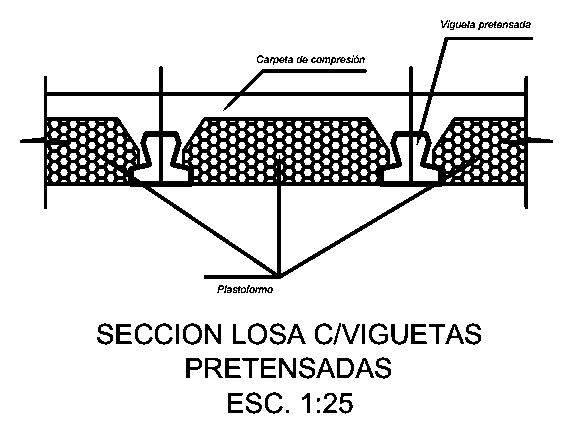
\includegraphics[width=0.60\linewidth]{plano02_seccion_losa_viguetas}
\nota{Tomado del Plano~02 del proyecto «Construcción Edificio de Posgrado» de la UATF.}
\end{figure}

\begin{figure}[H]
\centering
\caption{Corte transversal de la losa con la carpeta de compresión y la armadura de distribución}
\label{fig:corte}
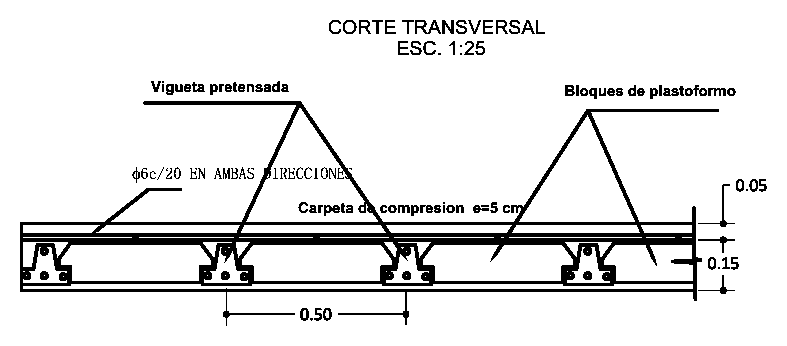
\includegraphics[width=0.85\linewidth]{plano02_corte_transversal}
\nota{Tomado del Plano~02 del proyecto. El corte acota 0,15~m de altura de complemento y 0,05~m de carpeta, mientras que las especificaciones técnicas y el certificado del fabricante indican 20~+~5~cm. Esta discrepancia se analiza en la sección~\ref{sec:analisis-documental}.}
\end{figure}

\subsection{Proceso constructivo}
\guia{Describir la secuencia de ejecución:
\begin{enumerate}
  \item replanteo;
  \item apuntalamiento y encofrado de vigas;
  \item colocación de viguetas y complementos;
  \item nervios transversales;
  \item armadura de distribución y de momentos negativos;
  \item instalaciones embebidas (ductos y cajas eléctricas y sanitarias);
  \item limpieza y humedecido;
  \item hormigonado y vibrado;
  \item curado;
  \item desapuntalamiento.
\end{enumerate}
Para cada actividad, indicar los puntos críticos de calidad. Usar el manual del fabricante y las especificaciones técnicas.}

\subsection{Consumos teóricos de materiales por metro cuadrado}
\guia{Calcular con los planos (Plano~03: cantidad de viguetas por paño) y la sección típica:
\begin{itemize}
  \item metros de vigueta por \mdos{};
  \item piezas de complemento por \mdos{};
  \item volumen de hormigón por \mdos{} (carpeta + nervios);
  \item kilogramos de acero por \mdos{} (malla de $\phi$6~c/20 + negativos + nervios).
\end{itemize}
Estos valores son la «cantidad teórica» del índice de desperdicio. Como referencia, el cómputo de acero de la losa de la obra da 4.171,18~kg para 1.109,84~\mdos{}, es decir, $\approx$~3,76~kg/\mdos{} \parencite{uatf_pao3}.}

\subsection{Defectos y fallas frecuentes}
\guia{Fisuras, flechas excesivas, segregación y nidos de grava, recubrimiento insuficiente, viguetas dañadas, desplazamiento de complementos durante el vaciado y falta de continuidad de la armadura negativa. Indicar sus causas y cómo prevenirlos.}

% ---------------------------------------------------------------------
\section{Marco normativo}

\subsection{Normas de gestión de la calidad}
\guia{ISO~9000:2026 y NB/ISO~9000:2026 (fundamentos y vocabulario); ISO~9001:2026 y NB/ISO~9001:2026 (requisitos; sustituyen a la edición 2015, cuyos certificados tienen un periodo de transición); ISO~10005:2018 y NB/ISO~10005:2021 (planes de la calidad); ISO~10006:2017 y NB/ISO~10006:2021 (calidad en proyectos); ISO~10014:2021 y NB/ISO~10014:2022 (beneficios financieros y económicos de la calidad).}

\subsection{Normas de hormigón estructural}
\guia{La CBH-87, citada en las especificaciones del proyecto, sigue siendo la norma de hormigón declarada obligatoria por decreto (D.~S.~22976 de 1991). La norma técnica actual es la NB~1225001-1:2017 (IBNORCA), basada en el código ACI~318 y ratificada por el MOPSV en 2020, aún no elevada a decreto supremo \pendiente{confirmar}. Declarar qué criterio de aceptación del hormigón se adopta y por qué. Código ACI~318-25 \parencite{aci318_2025}: capítulo~26 (documentos de construcción e inspección), muestreo (26.12.2), criterios de aceptación (26.12.3) y curado (26.5.3).}

\subsection{Norma de viguetas pretensadas}
\guia{NB~997:2016, «Elementos prefabricados de hormigón -- Viguetas prefabricadas de hormigón pretensado -- Requisitos y métodos de ensayo» (IBNORCA), citada en el certificado del fabricante \parencite{pretensa2025}. Usarla para los criterios de recepción de viguetas.}

\subsection{Normas de ensayo}
\guia{ASTM C172 (muestreo del hormigón fresco), C31 (elaboración y curado de probetas en obra), C143 (asentamiento), C39 (resistencia a compresión de cilindros), C94 (hormigón premezclado, si corresponde) y A615 (barras corrugadas), junto con sus equivalentes bolivianas: NB~634 (toma de muestras), NB~586 (probetas), NB~589 (cono de Abrams), NB~639 (compresión) y NB~736 y NB~739 (barras de acero) \pendiente{verificar equivalencias y años}. Indicar qué controla cada una en la losa.}

\subsection{Normativa de contratación pública}
\guia{Ley~1178 (SAFCO) y D.~S.~0181 (NB-SABS): funciones de la Supervisión y la Fiscalización, Libro de Órdenes, planillas de avance, órdenes de cambio, contratos modificatorios y sus límites porcentuales, y resolución de contrato. Según el artículo 89 del D.~S.~0181, los contratos modificatorios no pueden superar el 10~\% del monto del contrato y las órdenes de cambio el 5~\% (15~\% en conjunto en licitación pública). Incluir los decretos de ajuste excepcional de precios (D.~S.~5321 de 2025 y D.~S.~5597 de 2026). Relacionar con los hechos del caso (contrato modificatorio del 7,22~\% y resolución).}

% ---------------------------------------------------------------------
\section{Control de costos en obras públicas}
\guia{Análisis de precios unitarios (materiales, mano de obra, equipo, gastos generales, utilidad e impuestos), cómputos métricos, planillas de avance y certificados de pago. Explicar cómo el desperdicio y los reprocesos afectan al costo real frente al costo contractual. Mencionar el reajuste de precios por alza de insumos (2025--2026).}

% ---------------------------------------------------------------------
\section{Herramientas de la calidad}
\guia{Hoja de verificación, diagrama de Pareto, diagrama de Ishikawa, histograma, cartas de control, plan de puntos de inspección (PPI) y técnica 5W2H. Para cada una: para qué sirve y cómo se aplicará en esta tesis.}

% ---------------------------------------------------------------------
\section{Definición de términos básicos}
\guia{Glosario breve: calidad, conformidad, no conformidad, acción correctiva, desperdicio, reproceso, punto de inspección, liberación de actividad, trazabilidad, lote, f'c, asentamiento, carpeta de compresión, vigueta pretensada, complemento y apuntalamiento.}

% =====================================================================
%  CAPÍTULO 2. DISEÑO E IMPLEMENTACIÓN DEL MODELO (SGC)
%  Estructura del modelo científico según el Taller 4:
%  conceptualización y alcance -> factores y variables -> procedimiento
%  y toma de observaciones -> validación -> contraste de hipótesis.
% =====================================================================
\chapter{DISEÑO E IMPLEMENTACIÓN DEL SISTEMA DE GESTIÓN DE LA CALIDAD}
\label{cap:diseno}

% ---------------------------------------------------------------------
\section{Conceptualización y alcance del modelo de investigación}

El modelo de investigación compara el desempeño del proceso constructivo de la losa alivianada en dos condiciones:
\begin{itemize}
  \item sin un sistema de gestión de la calidad (primera losa, ya ejecutada), y
  \item con el SGC propuesto (segunda losa).
\end{itemize}
El efecto se mide mediante el costo unitario, el desperdicio de materiales y el costo de no calidad (Figura~\ref{fig:modelo} y Tabla~\ref{tab:fases}).

\begin{figure}[H]
\centering
\caption{Esquema del modelo de investigación}
\label{fig:modelo}
\begin{tikzpicture}[
  caja/.style={draw, rounded corners=2pt, align=center, text width=3.4cm,
               minimum height=2.1cm, font=\small, fill=gray!8},
  flecha/.style={-{Stealth[length=3mm]}, thick}]
  \node[caja] (o1) {\textbf{$O_1$: línea base}\\ Primera losa\\ sin SGC\\ 41 paños\\ 1.109,84~\mdos{}};
  \node[caja, right=0.4cm of o1] (x) {\textbf{$X$: aplicación}\\ \textbf{del SGC}\\ Plan de la calidad,\\ PPI y control\\ de materiales};
  \node[caja, right=0.4cm of x] (o2) {\textbf{$O_2$: posprueba}\\ Segunda losa\\ con SGC\\ (o simulación\\ \emph{ex ante})};
  \node[caja, right=0.4cm of o2] (h) {\textbf{Contraste}\\ Prueba \emph{t}\\ o Wilcoxon\\ $\alpha = 0{,}05$};
  \draw[flecha] (o1) -- (x);
  \draw[flecha] (x) -- (o2);
  \draw[flecha] (o2) -- (h);
\end{tikzpicture}
\nota{Elaboración propia.}
\end{figure}

\begin{table}[H]
\caption{Fases del modelo de investigación}
\label{tab:fases}
\begin{tabularx}{\linewidth}{@{}P{3.0cm}LP{4.0cm}P{1.7cm}@{}}
\toprule
\textbf{Fase} & \textbf{Actividades} & \textbf{Productos} & \textbf{Objetivo} \\
\midrule
1. Diagnóstico & Análisis documental, diagnóstico de brechas ISO~9001 y entrevistas & No conformidades y causas & OE1 \\
2. Línea base ($O_1$) & Cuantificación de consumos, desperdicios y costos de la primera losa & Índices de desperdicio y costo de no calidad & OE2 \\
3. Diseño ($X$) & Plan de la calidad, PPI, procedimientos y formatos & SGC del ítem & OE3 \\
4. Aplicación ($O_2$) & Implementación en la segunda losa o simulación & Índices con el SGC & OE4 \\
5. Contraste y validación & Pruebas estadísticas y juicio de expertos & Aceptación o rechazo de la hipótesis & OE5 \\
\bottomrule
\end{tabularx}
\nota{Elaboración propia.}
\end{table}

% ---------------------------------------------------------------------
\section{Caracterización del caso de estudio}

\subsection{Ubicación y descripción del edificio}
El Edificio de Posgrado se emplaza en la Ciudadela Universitaria de la UATF, en el sector noreste, junto al edificio del Vicerrectorado, sobre la avenida Las Banderas de la ciudad de Potosí, a 3650~m~s.~n.~m. El proyecto tiene seis niveles. Por el desnivel del terreno, la planta baja presenta desniveles en tres sectores. La fase en estudio comprende la obra gruesa (fundaciones, columnas, vigas, losas alivianadas y escaleras de hormigón armado) hasta la tercera losa. También incluye la colocación de ductos y cajas eléctricas y sanitarias embebidas en losas y vigas \parencite{uatf_item13}.

\subsection{Datos contractuales y cronología}

\begin{table}[H]
\caption{Cronología de la ejecución del proyecto}
\label{tab:cronologia}
\begin{tabularx}{\linewidth}{@{}P{3.2cm}L@{}}
\toprule
\textbf{Fecha} & \textbf{Hecho} \\
\midrule
06/05/2025 & Inicio de obra; plazo de 270 días calendario y monto de Bs~3.367.031,95. \\
12/06/2025 & FANCESA comunica la paralización temporal de su producción por falta de diésel. \\
04/09/2025 -- 08/12/2025 & Periodo de la Planilla de avance N.\textsuperscript{o}~2 (95 días trabajados). \\
09/10/2025 & Pronunciamiento de la Cámara de la Construcción de Tarija sobre el alza del cemento. \\
27/11/2025 & Certificados de calidad de viguetas pretensadas (PRETENSA) y de plastoformo (UNICON). \\
05/12/2025 & Certificado de laboratorio N.\textsuperscript{o}~000293 (probetas de columnas y vigas). \\
08/12/2025 & Avance acumulado del 56,97~\%; contrato modificado a Bs~3.610.125,43 y plazo de 360 días. \\
05/01 y 10/02 \pendiente{año} & Paralización por solicitud de resolución concertada del contrato y respuesta favorable de la UATF. \\
Planilla N.\textsuperscript{o}~3 & Resolución del contrato: avance del 57,48~\% y 1.109,84~\mdos{} de losa ejecutados. \\
\bottomrule
\end{tabularx}
\nota{Elaborado con base en \textcite{uatf2025pao2}, \textcite{uatf_pao3}, \textcite{uatf_item13}, \textcite{fancesa2025} y \textcite{cadeco2025}.}
\end{table}

\subsection{Sistema de losa: planos, especificaciones y certificados}
La primera losa se divide en 41 paños, de 1,40 a 52,38~\mdos{} cada uno, que suman 1.109,84~\mdos{} (Figura~\ref{fig:geometria}). Las características del sistema según los documentos del proyecto se resumen en la Tabla~\ref{tab:sistema}.

\begin{figure}[H]
\centering
\caption{Geometría y paños de la primera losa del Edificio de Posgrado}
\label{fig:geometria}
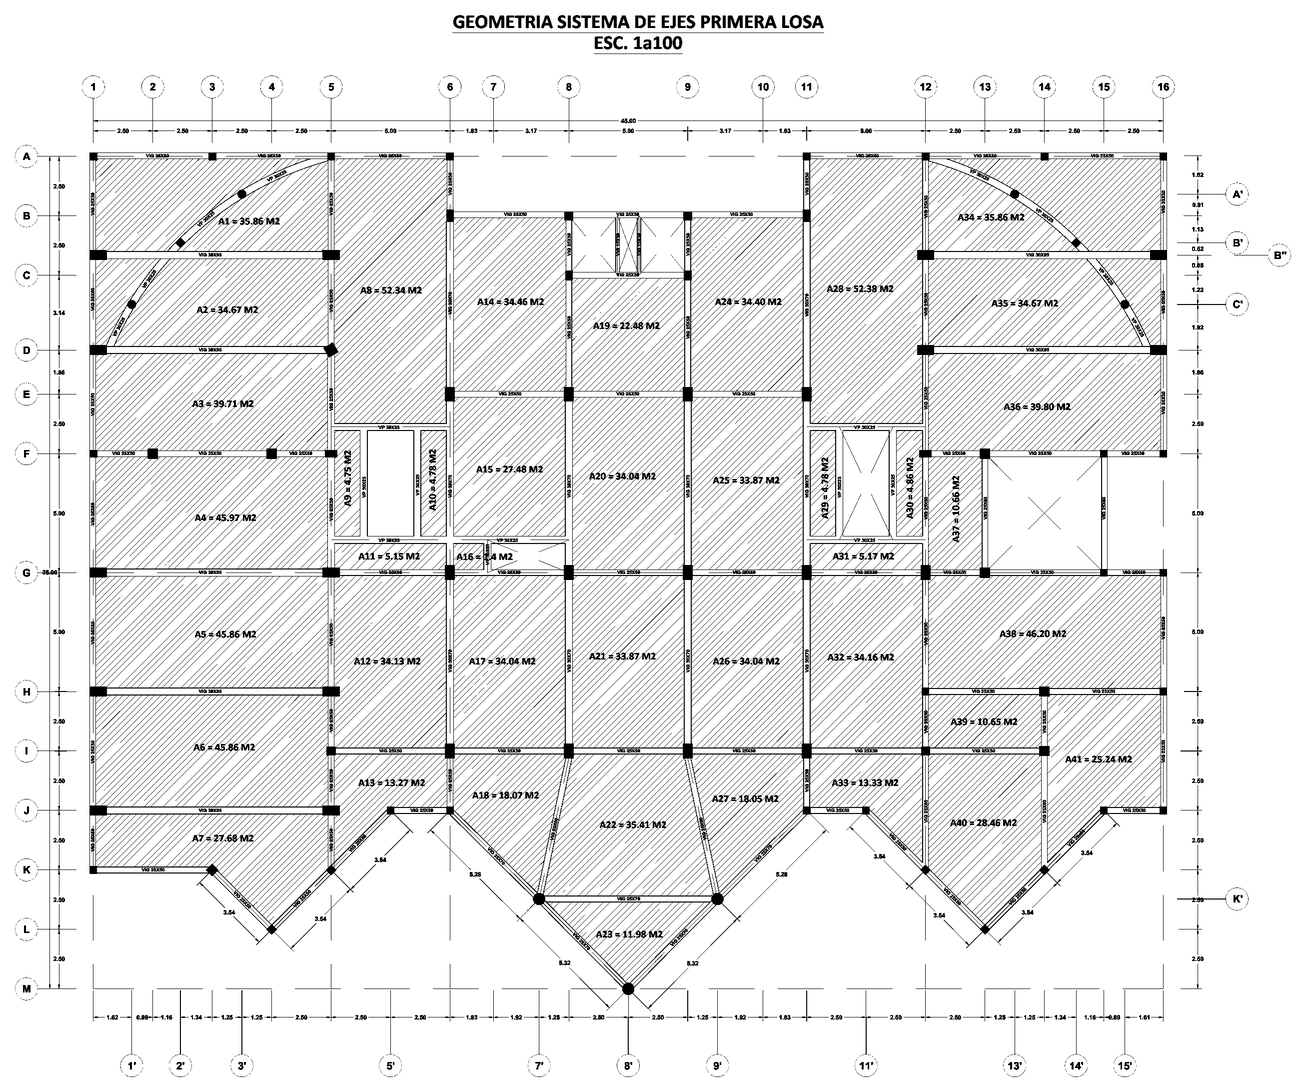
\includegraphics[width=\linewidth]{plano01_geometria_primera_losa}
\nota{Tomado del Plano~01 «Geometría sistema de ejes primera losa» (escala original 1:100). Las áreas A1 a A41 corresponden a los paños de losa computados.}
\end{figure}

\begin{table}[H]
\caption{Características de la losa alivianada según los documentos del proyecto}
\label{tab:sistema}
\begin{tabularx}{\linewidth}{@{}P{4.2cm}LP{3.6cm}@{}}
\toprule
\textbf{Característica} & \textbf{Valor} & \textbf{Fuente} \\
\midrule
Espesor total & 25~cm (20~cm + 5~cm de carpeta) & ET; certificado PRETENSA \\
Separación entre ejes de viguetas & 50~cm & Certificado PRETENSA \\
Luz máxima de vigueta & 7,50~m (simplemente apoyada) & Certificado PRETENSA \\
Sobrecarga admisible & 400~kg/\mdos{} & Certificado PRETENSA \\
Hormigón de viguetas & 350 a 400~kg/cm\textsuperscript{2} & ET \\
Hormigón de carpeta y nervios & H25, f'c~=~250~kg/cm\textsuperscript{2}, cemento $\geq$~400~kg/\mtres{} & ET \\
Armadura de distribución & $\phi$6~c/20~cm en ambas direcciones & Plano~02 \\
Complemento (según ET) & Plastoformo de 100~$\times$~50~$\times$~20~cm & ET \\
Complemento (suministrado) & Plastobloq de 20~$\times$~100~$\times$~44~cm, densidad 10~kg/\mtres{} & Certificado UNICON \\
\bottomrule
\end{tabularx}
\nota{ET: especificaciones técnicas del proyecto \parencite{uatf_et}. Certificados: \textcite{pretensa2025} y \textcite{unicon2025}.}
\end{table}

% ---------------------------------------------------------------------
\section{Definición de factores y variables}
\label{sec:variables}

Las variables, sus dimensiones e indicadores se detallan en el Anexo~\ref{anx:operacionalizacion}. Los indicadores principales se calculan de la siguiente manera.

\textbf{Índice de desperdicio del material $i$:}
\begin{equation}
  IDM_i = \frac{Q_{\text{real},i} - Q_{\text{teórica},i}}{Q_{\text{teórica},i}} \times 100
  \label{eq:idm}
\end{equation}
donde $Q_{\text{real},i}$ es la cantidad consumida (entregada menos sobrante recuperable) y $Q_{\text{teórica},i}$ es la cantidad según planos y cómputos.

\textbf{Costo unitario a precios constantes del contrato:}
\begin{equation}
  CU = \frac{\sum_{j} Q_{j}\, p_{j} + C_{MO} + C_{EQ}}{A}
  \label{eq:cu}
\end{equation}
donde $Q_j$ es la cantidad real del insumo $j$, $p_j$ su precio en el análisis de precios unitarios del contrato, $C_{MO}$ y $C_{EQ}$ los costos de mano de obra y equipo, y $A$ la superficie ejecutada (\mdos{}).

\textbf{Costo de la calidad y costo de no calidad (modelo PAF):}
\begin{equation}
  CC = C_{P} + C_{E}, \qquad CNC = C_{FI} + C_{FE}, \qquad \%CNC = \frac{CNC}{C_{\text{ítem}}} \times 100
  \label{eq:cnc}
\end{equation}
donde $C_P$ son los costos de prevención, $C_E$ los de evaluación, $C_{FI}$ los de fallas internas (desperdicio, retrabajo y reparaciones) y $C_{FE}$ los de fallas externas (sobremediciones corregidas, ampliaciones y multas).

\textbf{Reducción relativa del costo en el paño homólogo $k$:}
\begin{equation}
  r_k = \frac{CU_{\text{sin},k} - CU_{\text{con},k}}{CU_{\text{sin},k}}
  \label{eq:reduccion}
\end{equation}

\guia{Si un material solo puede medirse por vaciado o por losa completa (por ejemplo, el hormigón), la unidad de análisis de ese indicador será el vaciado y no el paño.}

% ---------------------------------------------------------------------
\section{Población y muestra}
La población está formada por las losas alivianadas del edificio (3.344,44~\mdos{}). La unidad de análisis es el paño de losa. Se adopta una muestra no probabilística censal: los 41 paños de la primera losa (preprueba) y los paños homólogos de la segunda losa (posprueba). Así se compara cada paño con otro de la misma geometría.

\guia{Confirmar con los planos de la segunda losa que los paños son homólogos (misma geometría y cantidad de viguetas). Si no lo son, comparar con muestras independientes (prueba \emph{t} para muestras independientes o U de Mann-Whitney).}

% ---------------------------------------------------------------------
\section{Diagnóstico de la situación actual (línea base)}

\subsection{Diagnóstico de brechas frente a la norma ISO~9001:2026}
\guia{Aplicar la lista de verificación (Anexo~\ref{anx:instrumentos}) a la contratista y a la Supervisión. Calificar cada requisito aplicable de las cláusulas 4 a 10 (cumple, cumple parcialmente o no cumple) y calcular el porcentaje de cumplimiento por cláusula. Presentar los resultados en una tabla y un gráfico de barras.}

\subsection{Análisis documental de la primera losa}
\label{sec:analisis-documental}

La revisión preliminar de los documentos de la obra muestra los siguientes hallazgos.

\textbf{a) Control de la resistencia del hormigón.} El certificado de laboratorio N.\textsuperscript{o}~000293 (Tabla~\ref{tab:probetas}) es el único registro de ensayos de compresión adjunto a la Planilla N.\textsuperscript{o}~2. Comprende doce probetas de 15~$\times$~30~cm (6~$\times$~12~pulg) de columnas y vigas, ensayadas entre los 55 y 76 días y «proyectadas» a 28 días con un factor de tiempo \parencite{labuatf2025}. Todos los valores superan f'c~=~250~kg/cm\textsuperscript{2}. Sin embargo:
\begin{enumerate*}[label=(\roman*)]
  \item no hay probetas de la losa alivianada;
  \item los ensayos no se hicieron a la edad especificada de 28 días;
  \item las probetas fueron elaboradas por la propia contratista, sin muestreo independiente; y
  \item cuatro de los doce valores proyectados están por debajo de 260~kg/cm\textsuperscript{2}, con poco margen sobre la resistencia especificada.
\end{enumerate*}

\begin{table}[H]
\caption{Resultados del certificado de laboratorio N.\textsuperscript{o}~000293}
\label{tab:probetas}
\begin{tabularx}{\linewidth}{@{}LQ{1.6cm}Q{1.9cm}Q{3.0cm}Q{1.3cm}Q{1.0cm}Q{1.0cm}@{}}
\toprule
\textbf{Elemento} & \textbf{N.\textsuperscript{o} probetas} & \textbf{Edad (días)} & \textbf{Resistencia proyectada a 28 días (kg/cm\textsuperscript{2})} & \textbf{Media} & \textbf{$s$} & \textbf{CV} \\
\midrule
Columnas & 10 & 55--76 & 253,6 -- 287,8 & 267,2 & 9,9 & 3,7~\% \\
Vigas & 2 & 76 & 252,0 -- 261,4 & 256,7 & 6,6 & 2,6~\% \\
Losa alivianada & 0 & --- & sin ensayos & --- & --- & --- \\
\bottomrule
\end{tabularx}
\nota{Elaborado con base en el certificado del Laboratorio de Resistencia de Materiales y Tecnología del Hormigón de la Carrera de Ingeniería Civil de la UATF \parencite{labuatf2025}. $s$: desviación estándar; CV: coeficiente de variación.}
\end{table}

\textbf{b) Requerimientos de la Supervisión.} En su informe de la Planilla N.\textsuperscript{o}~2, la Supervisión recomendó a la contratista \parencite{uatf2025pao2}:
\begin{itemize}
  \item presentar las garantías de todos los materiales empleados;
  \item realizar la rotura de probetas de los elementos vaciados;
  \item presentar las dosificaciones de los hormigones.
\end{itemize}
Es decir, al cierre del periodo no se contaba con estos controles básicos.

\textbf{c) Coherencia de los documentos técnicos.} Tres documentos describen el complemento de manera distinta:
\begin{itemize}
  \item las especificaciones técnicas exigen bloques de 100~$\times$~50~$\times$~20~cm;
  \item el corte transversal del Plano~02 acota una altura de 0,15~m;
  \item el certificado del proveedor corresponde a bloques de 20~$\times$~100~$\times$~44~cm \parencite{uatf_et,unicon2025}.
\end{itemize}
La falta de control de la información documentada y de los cambios, que exige la norma ISO~9001, es una no conformidad del sistema actual.

\textbf{d) Cantidades de materiales.} Se entregaron 2.350 piezas de plastoformo \parencite{unicon2025}. Con una separación de 50~cm entre ejes y bloques de 1,00~m de largo, el consumo teórico bruto es de 2 piezas por \mdos{}, es decir, $\approx$~2.220 piezas para 1.109,84~\mdos{} sin descontar nervios ni bordes. La diferencia preliminar es de $\approx$~130 piezas ($\approx$~6~\%).

Además, el cómputo de acero de la planilla de resolución incluye «losa alivianada: 3 $\times$ 4.171,18 kg = 12.513,54 kg», aunque solo se ejecutó una losa \parencite{uatf_pao3}.

\pendiente{verificar con la Supervisión si las 2.350 piezas corresponden solo a la primera losa, el número real de piezas colocadas y sobrantes, y a qué corresponde el factor 3 del acero.}

\subsection{No conformidades y análisis de causas}
\guia{Registrar las no conformidades encontradas en el Libro de Órdenes (fotocopias en la Planilla N.\textsuperscript{o}~2), en los informes de Supervisión y en las entrevistas. Clasificarlas por categoría: materiales, mano de obra, método, documentación, equipo y medición. Elaborar un diagrama de Pareto (frecuencia y costo) y un diagrama de Ishikawa de las causas del desperdicio y de los sobrecostos.}

\subsection{Cuantificación del desperdicio de materiales y del costo de no calidad}
\guia{Aplicar las ecuaciones \eqref{eq:idm} a \eqref{eq:cnc} a la primera losa:
\begin{enumerate}
  \item Cantidades teóricas: planos 01 a 03 y cómputos.
  \item Cantidades entregadas: notas de entrega, facturas y kardex.
  \item Cantidades pagadas: planillas de avance.
\end{enumerate}
Presentar una tabla por material (hormigón, acero, viguetas y plastoformo) con el índice de desperdicio y su costo a precios del contrato. Este es el valor de referencia ($O_1$) de la hipótesis.}

% =====================================================================
%  CAPÍTULO 3. PRESENTACIÓN DE RESULTADOS Y ANÁLISIS DE LOS MISMOS
% =====================================================================
\chapter{PRESENTACIÓN DE RESULTADOS Y ANÁLISIS DE LOS MISMOS}
\label{cap:resultados}

\guia{Según el Taller 5, los resultados se presentan en tablas y gráficos fáciles de entender. Se describen en pasado, en párrafos y sin juicios de valor, y responden a cada objetivo con la metodología de análisis definida. La interpretación y el contraste con la teoría y los antecedentes van en la sección de discusión.}

% ---------------------------------------------------------------------
\section{Resultados del diagnóstico y de la línea base}
\guia{OE1 y OE2. Porcentaje de cumplimiento de la norma ISO~9001:2026 por cláusula (gráfico de barras); no conformidades por categoría (Pareto); diagrama de Ishikawa; tabla de índices de desperdicio y costo de no calidad de la primera losa por material.}

% ---------------------------------------------------------------------
\section{Resultados de la aplicación del SGC en el control de materiales}
\guia{OE4. Índice de desperdicio por material y por paño en la segunda losa, comparado con la línea base (tabla y gráfico de barras agrupadas). Porcentaje de lotes conformes y de paños liberados sin observaciones.}

% ---------------------------------------------------------------------
\section{Resultados del control de calidad de materiales y del hormigón}
\guia{Resultados de asentamiento y de resistencia a compresión a 28 días de la losa: media, desviación estándar, coeficiente de variación y cumplimiento de los criterios de aceptación (sección~\ref{sec:contraste} y Tabla~\ref{tab:ppi}). Comparar con los resultados de la línea base (Tabla~\ref{tab:probetas}).}

% ---------------------------------------------------------------------
\section{Resultados de costos}
\guia{Costo unitario con y sin SGC a precios constantes (ecuación~\ref{eq:cu}), comparado con el precio contractual de Bs~215,68/\mdos{}. Costos de la calidad y de no calidad (ecuación~\ref{eq:cnc}). Ahorro proyectado en el saldo de 2.234,60~\mdos{}.}

% ---------------------------------------------------------------------
\section{Contraste de hipótesis}
\guia{Para cada hipótesis presentar: estadístico de prueba, valor $p$, decisión (se rechaza o no $H_0$) y conclusión en palabras. Incluir la prueba de normalidad.}

% ---------------------------------------------------------------------
\section{Validación del SGC por juicio de expertos}
\guia{Tabla con el coeficiente V de Aiken por criterio (pertinencia, claridad, suficiencia y aplicabilidad) y las observaciones de los expertos incorporadas al SGC.}

% ---------------------------------------------------------------------
\section{Discusión de resultados}
\guia{Contrastar los resultados con los antecedentes y el marco teórico. ¿Los índices de desperdicio y la reducción de costos son coherentes con lo reportado en otras investigaciones? Explicar las coincidencias y las diferencias, las limitaciones del estudio y el alcance de la validez de los resultados.}

% =====================================================================
%  CONCLUSIONES Y RECOMENDACIONES
% =====================================================================
\chapter*{Conclusiones y recomendaciones}
\addcontentsline{toc}{chapter}{CONCLUSIONES Y RECOMENDACIONES}
\setcounter{section}{0}
\renewcommand{\thesection}{\arabic{section}}

\guia{Las conclusiones vinculan el desarrollo del trabajo con la pregunta del problema. Debe haber una conclusión por cada objetivo específico, y la conclusión general debe decir si se acepta o se rechaza la hipótesis, con los indicadores que lo demuestran. También se señalan las debilidades del estudio (Talleres 5 y 6).}

\section{Conclusión general}
\pendiente{responder el problema general e indicar si se acepta o se rechaza la hipótesis, con la reducción de costo obtenida.}

\section{Conclusiones específicas}
\begin{enumerate}[label=\textbf{\arabic*.}]
  \item \textbf{(OE1)} \pendiente{estado de la gestión de la calidad y no conformidades principales.}
  \item \textbf{(OE2)} \pendiente{línea base: índices de desperdicio y costo de no calidad de la primera losa.}
  \item \textbf{(OE3)} \pendiente{componentes del SGC diseñado.}
  \item \textbf{(OE4)} \pendiente{efecto del SGC en el costo unitario y en el desperdicio.}
  \item \textbf{(OE5)} \pendiente{resultado de las pruebas estadísticas y de la validación por expertos.}
\end{enumerate}

\section{Recomendaciones}
\guia{Recomendaciones para el Departamento de Infraestructura de la UATF, para la Supervisión y la Fiscalización, para futuras empresas contratistas y para futuras investigaciones (variables no estudiadas, otros ítems, otras obras).}

\renewcommand{\thesection}{\thechapter.\arabic{section}}


% ---------------- Bibliografía (APA 7.ª ed., orden alfabético)
\printbibliography[heading=bibintoc,title={Bibliografía}]

% ---------------- Anexos
% =====================================================================
%  ANEXOS
% =====================================================================
\appendix
\addtocontents{toc}{\protect\renewcommand{\protect\cftchappresnum}{\appendixname\ }}
\chapter*{Anexos}
\phantomsection\addcontentsline{toc}{chapter}{ANEXOS}

% ---------------------------------------------------------------------
\begin{landscape}
\chapter{MATRIZ DE CONSISTENCIA}
\label{anx:matriz}
\begingroup\small\setstretch{1}
\begin{longtable}{@{}P{4.4cm}P{4.4cm}P{4.6cm}P{4.0cm}P{4.3cm}@{}}
\caption{Matriz de consistencia de la investigación}\label{tab:matriz-consistencia}\\
\toprule
\textbf{Problema} & \textbf{Objetivos} & \textbf{Hipótesis} & \textbf{Variables e indicadores} & \textbf{Metodología} \\
\midrule
\endfirsthead
\multicolumn{5}{@{}l}{\textit{(continuación)}}\\
\toprule
\textbf{Problema} & \textbf{Objetivos} & \textbf{Hipótesis} & \textbf{Variables e indicadores} & \textbf{Metodología} \\
\midrule
\endhead
\bottomrule
\endfoot
\textbf{General:} ¿De qué manera un Sistema de Gestión de la Calidad basado en la norma ISO~9001, centrado en el control de materiales, permite reducir los costos de ejecución de las losas alivianadas con viguetas pretensadas del Edificio de Posgrado de la Universidad Autónoma Tomás Frías?
& \textbf{General:} Diseñar un Sistema de Gestión de la Calidad basado en la norma ISO~9001, centrado en el control de materiales, para reducir los costos de ejecución de las losas alivianadas con viguetas pretensadas del Edificio de Posgrado de la Universidad Autónoma Tomás Frías.
& \textbf{HG:} La aplicación de un Sistema de Gestión de la Calidad basado en la norma ISO~9001, centrado en el control de materiales, reduce en al menos un 5~\% el costo unitario de ejecución (Bs/\mdos{}, a precios constantes del contrato) de las losas alivianadas con viguetas pretensadas del Edificio de Posgrado de la UATF, respecto de la línea base de la primera losa.
& \textbf{X:} SGC (planificación de la calidad, control de materiales, control del proceso, seguimiento y mejora). \newline \textbf{Y:} costo de ejecución de la losa (costo directo, desperdicio, costo de no calidad, costo de la calidad, conformidad del hormigón). \newline \textbf{Interviniente controlada:} precios (constantes del contrato).
& Tipo aplicada; enfoque cuantitativo; nivel explicativo, con fase descriptiva y componente propositivo. Diseño no experimental: línea base retrospectiva y documental de la primera losa ($O_1$), SGC diseñado ($X$) y evaluación \emph{ex ante} ($O_2$ simulado) con un modelo de costos y una simulación de Monte Carlo de \MCiter{} iteraciones. Se acepta $H_1$ si $P \ge 0{,}95$ ($\alpha = 0{,}05$). \\
\midrule
\textbf{PE1:} ¿Cómo se gestionaron la calidad y el control de materiales en la ejecución de la primera losa alivianada del Edificio de Posgrado?
& \textbf{OE1:} Caracterizar la gestión de la calidad y el control de materiales aplicados en la ejecución de la primera losa alivianada (1.109,84~\mdos{}) e identificar las no conformidades y sus causas.
& Descriptivo (sin hipótesis).
& Porcentaje de cumplimiento de los requisitos ISO~9001:2026 por cláusula; número de no conformidades y sus causas.
& Análisis documental (planillas, Libro de Órdenes, certificados, contrato, planos y ET); lista de verificación C.1; Pareto e Ishikawa. \\
\midrule
\textbf{PE2:} ¿Cuál es el nivel de desperdicio de materiales (hormigón, acero, viguetas pretensadas y plastoformo) y cuál es el costo de no calidad de la primera losa?
& \textbf{OE2:} Cuantificar la línea base del índice de desperdicio de materiales (hormigón, acero, viguetas pretensadas y plastoformo) y del costo de no calidad de la primera losa. Para ello se compararán las cantidades teóricas, adquiridas y pagadas.
& Descriptivo: valores de referencia de la línea base.
& $IDM_i$ (ecuación~\eqref{eq:idm}); costo de no calidad en Bs/\mdos{} y en \% del costo unitario.
& Cantidades teóricas por paño (Planos 01 a 03) frente a las cantidades entregadas y pagadas (certificados y planillas); rangos de la literatura cuando no hubo registros. \\
\midrule
\textbf{PE3:} ¿Qué componentes debe tener un SGC para el proceso constructivo de losas alivianadas con viguetas pretensadas?
& \textbf{OE3:} Establecer los componentes del SGC: plan de la calidad, plan de puntos de inspección y ensayo (PPI), procedimientos de control de materiales, gestión de no conformidades y registro de costos de la calidad. Se basarán en las normas ISO~9001:2026 e ISO~10005:2018, en la normativa de hormigón estructural y en los ensayos ASTM.
& Propositivo (sin hipótesis).
& Componentes del SGC: plan de la calidad, PPI, procedimientos PCM-01 a PCM-05, gestión de no conformidades y planilla de costos de la calidad.
& Diseño a partir de la ISO~9001:2026, la ISO~10005:2018, el ACI~318-25 (capítulo~26), la NB~997 y las normas ASTM; formatos C.2 a C.6. \\
\midrule
\textbf{PE4:} ¿En qué medida el SGC propuesto reduce el costo unitario y el desperdicio de materiales respecto de la línea base?
& \textbf{OE4:} Evaluar \emph{ex ante}, mediante un modelo de costos y simulación de Monte Carlo, el efecto del SGC sobre el costo unitario (Bs/\mdos{}) y el desperdicio de materiales de los 2.234,60~\mdos{} de losa restantes, respecto de la línea base. \newline \textbf{OE5:} Contrastar la hipótesis mediante reglas de decisión probabilísticas con $\alpha = 0{,}05$ y validar el SGC mediante juicio de expertos.
& \textbf{HE1:} El SGC reduce el índice de desperdicio de materiales de la losa con respecto a la línea base. \newline \textbf{HE2:} El SGC reduce el costo de no calidad (fallas internas y externas) del ítem con respecto a la línea base. \newline \textbf{HG} (fila general).
& Costo unitario (ecuación~\eqref{eq:cu-modelo}); costo de no calidad (ecuación~\eqref{eq:cnc-modelo}); $IDM$ ponderado; reducción relativa $r$ (ecuación~\eqref{eq:r-modelo}); coeficiente V de Aiken (ecuación~\eqref{eq:aiken}).
& Modelo de costos y simulación de Monte Carlo (Sección~\ref{sec:modelo-simulacion}); reglas de decisión de la Tabla~\ref{tab:reglas-decision}; sensibilidad y punto de equilibrio; validación por juicio de expertos con el formato C.8 (pendiente). \\
\end{longtable}
\endgroup
\nota{Elaboración propia. Las formulaciones del problema, los objetivos y las hipótesis son las de la Introducción.}

% ---------------------------------------------------------------------
\chapter{OPERACIONALIZACIÓN DE VARIABLES}
\label{anx:operacionalizacion}
\begingroup\small\setstretch{1}
\begin{longtable}{@{}P{2.4cm}P{3.0cm}P{4.6cm}P{3.6cm}P{3.3cm}P{4.6cm}@{}}
\caption{Operacionalización de las variables}\label{tab:operacionalizacion}\\
\toprule
\textbf{Variable} & \textbf{Dimensión} & \textbf{Indicador} & \textbf{Fórmula o unidad} & \textbf{Instrumento} & \textbf{Medición en esta tesis} \\
\midrule
\endfirsthead
\multicolumn{6}{@{}l}{\textit{(continuación)}}\\
\toprule
\textbf{Variable} & \textbf{Dimensión} & \textbf{Indicador} & \textbf{Fórmula o unidad} & \textbf{Instrumento} & \textbf{Medición en esta tesis} \\
\midrule
\endhead
\bottomrule
\endfoot
\textbf{X:} Sistema de Gestión de la Calidad
& Planificación de la calidad & Cumplimiento de los requisitos ISO~9001:2026 (cláusulas 4 a 10) & \% de requisitos cumplidos & Lista de verificación C.1 & Línea base documental; verificación futura en obra \\
& Control de materiales & Lotes recibidos con certificado o ensayo conforme & \% de lotes conformes & Ficha de recepción C.3 (PCM-01) & Verificación futura en obra \\
& & Conciliación de cantidades por paño (teórica, entregada, colocada y pagada) & Diferencia en \% & Ficha C.4 (PCM-02 a PCM-04) & Línea base documental; verificación futura \\
& Control del proceso (PPI) & Puntos de inspección ejecutados frente a programados & \% & Fichas PPI C.2 & Verificación futura en obra \\
& Seguimiento y mejora & No conformidades detectadas y cerradas & N.\textsuperscript{o}; \% cerradas; días de cierre & Registro de NC C.5 & Línea base documental; verificación futura \\
\midrule
\textbf{Y:} Costo de ejecución de la losa
& Costo directo & Costo unitario de ejecución & Bs/\mdos{} (ecuación~\eqref{eq:cu-modelo}) & APU de referencia (Anexo~\ref{anx:apu}) y modelo (Anexo~\ref{anx:modelo}) & Línea base calibrada; simulación \emph{ex ante} \\
& Desperdicio de materiales & Índice de desperdicio por material & $IDM_i$ (ecuación~\eqref{eq:idm}) & Ficha C.4; planillas y certificados & Línea base (EPS y acero documentados; viguetas y hormigón, literatura); simulación \emph{ex ante} \\
& Costo de no calidad & Pérdidas de materiales y retrabajos & Bs/\mdos{}; \% del costo unitario (ecuación~\eqref{eq:cnc-modelo}) & Planilla de costos de la calidad C.6; modelo & Simulación \emph{ex ante} \\
& Costo de la calidad & Costos de prevención y evaluación del SGC & Bs/\mdos{}; \% del costo unitario & Planilla C.6; modelo & Simulación \emph{ex ante} \\
& Conformidad del hormigón & Ensayos de aceptación conformes (ACI~318-25, 26.12.3.1) y frecuencia de muestreo & \% de ensayos conformes; n.\textsuperscript{o} de muestras (ecuación~\eqref{eq:nensayos}) & Ensayos ASTM C31, C39 y C143 & Línea base documental; verificación futura \\
& Efecto del SGC & Reducción relativa del costo unitario & $r$ en \% (ecuación~\eqref{eq:r-modelo}) & Modelo y simulación (Anexo~\ref{anx:modelo}) & Simulación \emph{ex ante} \\
\midrule
\textbf{Interviniente:} precios de los materiales
& Variación de precios 2025--2026 & Control de la variable & Precios constantes del contrato & --- & Controlada en el modelo \\
\end{longtable}
\endgroup
\nota{Elaboración propia. Los instrumentos C.1 a C.8 están en el Anexo~\ref{anx:instrumentos}. La verificación futura en obra sigue el protocolo de la Sección~\ref{sec:verificacion-futura}.}
\end{landscape}

% ---------------------------------------------------------------------
\IfFileExists{capitulos/91_anexo_instrumentos.tex}{% =====================================================================
%  ANEXO C. INSTRUMENTOS DE RECOLECCIÓN DE DATOS Y FORMATOS DEL SGC
%  C.1 (lista de verificación ISO 9001:2026) se incluye desde
%  capitulos/91a_lista_verificacion_iso9001.tex (otro archivo).
%  C.2 a C.8: formatos listos para imprimir (tamaño carta).
% =====================================================================
\chapter{INSTRUMENTOS DE RECOLECCIÓN DE DATOS Y FORMATOS DEL SGC}
\label{anx:instrumentos}

% --- Utilidades locales para los formatos -----------------------------
\providecommand{\casilla}{\framebox[1.9ex]{\rule{0pt}{1.3ex}}}
\providecommand{\campo}[1]{#1~\hrulefill}
\providecommand{\fila}{\rule{0pt}{0.58cm}}
\providecommand{\firma}[1]{\parbox[b]{3.7cm}{\centering\rule{0pt}{0.75cm}\rule{3.4cm}{0.4pt}\\[-1pt]{\scriptsize #1}}}
\newcommand{\cabeceraformato}[2]{%
  \par\noindent{\footnotesize\setstretch{1}%
  \renewcommand{\arraystretch}{1.35}%
  \begin{tabular}{@{}|p{0.30\linewidth}|p{0.44\linewidth}|p{0.183\linewidth}|@{}}
  \hline
  \textbf{UATF -- Edificio de Posgrado} & \multirow{2}{=}{\centering\textbf{#2}} & \textbf{Código:} #1 \\
  Ítem 13: losa alivianada h~=~25~cm & & Versión 0 \\
  \hline
  \end{tabular}\par}\smallskip}

Este anexo reúne los instrumentos de recolección de datos de la investigación y los formatos del Sistema de Gestión de la Calidad (SGC) propuesto en la Sección~\ref{sec:diseno-sgc}. Los formatos C.2 a C.6 son los registros del SGC: se imprimen en tamaño carta, se llenan en obra y se archivan por losa y por paño. Los instrumentos C.7 y C.8 sirven a la investigación: la guía de entrevista para el diagnóstico (OE1) y el formato de validación por juicio de expertos (OE5). La relación de cada formato con el sistema es la siguiente:

\begin{center}
\footnotesize\setstretch{1}\renewcommand{\arraystretch}{1.25}
\begin{tabularx}{\linewidth}{@{}P{1.0cm}LP{4.6cm}P{3.0cm}@{}}
\toprule
\textbf{Código} & \textbf{Formato o instrumento} & \textbf{Componente del SGC} & \textbf{Responsable} \\
\midrule
C.1 & Lista de verificación de requisitos ISO~9001:2026 & Diagnóstico y auditoría interna & Investigador; auditor \\
C.2 & Fichas PPI de liberación por paño & Plan de puntos de inspección (Tabla~\ref{tab:ppi}) & Encargado de calidad; Supervisor \\
C.3 & Ficha de recepción de materiales & PCM-01 (Tabla~\ref{tab:pcm01}) & Almacenero; encargado de calidad \\
C.4 & Control de materiales y conciliación por paño & PCM-02, PCM-03 y PCM-04 & Almacenero; encargado de calidad \\
C.5 & Registro de no conformidades y acción correctiva & PCM-05; procedimiento de NC & Encargado de calidad \\
C.6 & Planilla de costos de la calidad (PAF) & Registro de costos de la calidad & Encargado de calidad \\
C.7 & Guía de entrevista semiestructurada & Diagnóstico (OE1) & Investigador \\
C.8 & Formato de validación por juicio de expertos & Validación (OE5) & Investigador; expertos \\
\bottomrule
\end{tabularx}
\end{center}

\IfFileExists{capitulos/91a_lista_verificacion_iso9001.tex}{% =====================================================================
%  ANEXO C.1. LISTA DE VERIFICACIÓN DE REQUISITOS DE ISO 9001:2026
%  APLICADA (DOCUMENTALMENTE) A LA EJECUCIÓN DE LA PRIMERA LOSA
%  Se inserta dentro del Anexo C (capitulos/91_anexo_instrumentos.tex)
%  con \input{capitulos/91a_lista_verificacion_iso9001}.
%  Las calificaciones se reproducen en el script
%  03_Datos_Obra_Edificio_Posgrado/04_Extraccion_de_Datos/scripts/
%  cap2_diagnostico_figuras.py (Figura de brechas del Capítulo 2).
% =====================================================================
\section*{C.1. Lista de verificación de requisitos de ISO~9001:2026 aplicada a la ejecución de la primera losa}
\addcontentsline{toc}{section}{C.1. Lista de verificación de requisitos de ISO~9001:2026 (primera losa)}
\label{anx:lista-iso}

\textbf{Propósito y alcance.} La lista sirve para diagnosticar las brechas entre la gestión real del proceso constructivo de la losa alivianada y los requisitos de las cláusulas 4 a 10 de la norma ISO~9001:2026 \parencite{iso9001_2026}. Se aplicó a la ejecución de la primera losa (41 paños; 1.109,84~\mdos{}), entendida como el sistema formado por la empresa contratista, su Dirección de Obra y los controles de la Supervisión que constan en los documentos. Los requisitos se redactaron como paráfrasis del autor, en términos del proceso de la losa; no reproducen el texto de la norma. La numeración corresponde a la estructura de cláusulas que la edición de 2026 conserva de la de 2015. \pendiente{contrastar la numeración de las subcláusulas con el texto de la NB/ISO~9001:2026 de IBNORCA \parencite{ibnorca9001_2026}.}

\textbf{Método.} La aplicación fue documental y la realizó el investigador. Se revisaron, página por página, la Planilla de avance de obra N.\textsuperscript{o}~2 con sus anexos (informe de Supervisión, cómputos, certificados, contrato, Libro de Órdenes y cronogramas), la planilla y los cómputos de cierre por resolución del contrato, el expediente del ítem~13, las especificaciones técnicas y los planos 01 a 03. Cada requisito aplicable se calificó así: \textbf{1} = cumple (el requisito está establecido, se aplicó y hay evidencia documental); \textbf{0,5} = cumple parcialmente (hay evidencia de una aplicación parcial, informal o sin registros completos); \textbf{0} = no cumple (no se encontró evidencia en los documentos revisados, o la evidencia muestra lo contrario); \textbf{NA} = no aplica al proceso de la losa (se excluye del denominador). El porcentaje de cada cláusula es la suma de las calificaciones dividida entre el número de requisitos aplicables. La interpretación usa la escala de \textcite[p.~42]{mamanicalsina2025}: 0--25~\% deficiente o no implementado; 26--50~\% básico o en desarrollo; 51--75~\% aceptable; 76--100~\% excelente.

\textbf{Limitación.} Una calificación de 0 por falta de evidencia documental no prueba que la práctica no existiera; prueba que no quedó registrada. Las entrevistas de la guía C.7 a la Dirección de Obra, a la Supervisión y a la Fiscalización permitirán verificar o corregir estas calificaciones. Para las auditorías internas del SGC propuesto, la columna de requisitos se usa sin cambios y las columnas de evidencia y calificación se llenan en cada aplicación.

\begingroup\footnotesize\setstretch{1}\setlength{\tabcolsep}{3pt}
\begin{longtable}{@{}P{1.15cm}P{3.85cm}P{5.05cm}Q{0.85cm}P{4.15cm}@{}}
\caption{Lista de verificación C.1 aplicada a la ejecución de la primera losa}\label{tab:lista-iso}\\
\toprule
\textbf{Cláusula} & \textbf{Requisito (paráfrasis aplicada a la losa)} & \textbf{Evidencia documental encontrada} & \textbf{Calif.} & \textbf{Observación} \\
\midrule
\endfirsthead
\multicolumn{5}{@{}l}{\textit{(continuación)}}\\
\toprule
\textbf{Cláusula} & \textbf{Requisito (paráfrasis aplicada a la losa)} & \textbf{Evidencia documental encontrada} & \textbf{Calif.} & \textbf{Observación} \\
\midrule
\endhead
\midrule
\multicolumn{5}{@{}r}{\textit{(continúa)}}\\
\endfoot
\bottomrule
\endlastfoot
%
\multicolumn{5}{@{}l}{\textbf{4. Contexto de la organización}}\\
4.1 & Determinar las cuestiones externas e internas que afectan al proceso de la losa (abastecimiento, precios, clima y pertinencia del cambio climático) y darles seguimiento. & No hay análisis de contexto. Las lluvias (siete días) y la demora de materiales por escasez de combustible solo se anotaron después de ocurridas, para pedir ampliación de plazo (PAO2, pp.~114--124). & 0 & La escasez de diésel ya era pública en junio de 2025 (FANCESA; Las Lomas) y no generó previsiones. \\
4.2 & Identificar las partes interesadas pertinentes (UATF, Supervisión, Fiscalización, proveedores, laboratorio, usuarios) y sus requisitos. & El contrato define partes y obligaciones (PAO2, pp.~91--112); la ET y los planos fijan los requisitos del producto. No hay análisis de las demás partes interesadas. & 0,5 & Documentados solo los requisitos de la entidad contratante. \\
4.3 & Definir y documentar el alcance del sistema, con los requisitos que no se aplican y su justificación. & No existe un sistema declarado ni un documento de alcance; los 15 documentos de la planilla no incluyen un plan de la calidad (PAO2, pp.~3--4, 12). & 0 & --- \\
4.4 & Determinar los procesos de la losa (abastecimiento, montaje, armado, hormigonado, curado y medición) con entradas, salidas, secuencia, criterios, responsables y recursos. & La secuencia general figura en la ET (pp.~1--4) y en el cronograma A-8 (PAO2, p.~137); no hay mapa de procesos, procedimientos ni responsables por actividad. & 0,5 & El cronograma no refleja la secuencia real: la losa se armó en noviembre de 2025. \\
%
\multicolumn{5}{@{}l}{\textbf{5. Liderazgo}}\\
5.1.1 a & Demostrar el compromiso de la dirección de la empresa con la eficacia del sistema (rendición de cuentas, recursos, integración en los procesos). & La dirección de la empresa solo aparece en las cartas de entrega de planillas y en las firmas de cobro (PAO2, pp.~12, 14, 88). & 0 & --- \\
5.1.1 b & Promover una cultura de la calidad y un comportamiento ético en la ejecución, la medición y el registro de la obra. & No hay evidencia de acciones; las diferencias de cantidades del acero no tienen explicación documentada (PAO3, hoja de cómputos, filas 375--541; Exp., p.~12). & 0 & Énfasis de la edición 2026. Es ausencia de evidencia, no un juicio sobre las personas. \\
5.1.2 & Mantener el enfoque al cliente: cumplir los requisitos de la UATF y los legales, y atender los riesgos que afectan la conformidad de la losa. & Obra ejecutada con autorización de la Supervisión (PAO2, pp.~114--125), pero con retraso acumulado de 3,03~\% (p.~10) y con garantías, ensayos y dosificaciones pendientes al cierre del periodo (p.~9). & 0,5 & --- \\
5.2 & Establecer, comunicar y mantener disponible una política de la calidad apropiada al proyecto. & No se encontró. & 0 & --- \\
5.3 & Asignar y comunicar roles, responsabilidades y autoridades, incluido quién informa sobre el desempeño del sistema. & Director de Obra designado y evaluado (PAO2, p.~9); Supervisora y Fiscal designados (pp.~7, 127). No hay organigrama ni responsable de calidad; falta la constancia del Director de Obra en las 12 hojas del Libro de Órdenes (pp.~114--125). & 0,5 & Cl.~25.ª del contrato (PAO2, p.~100). \\
%
\multicolumn{5}{@{}l}{\textbf{6. Planificación}}\\
6.1 a & Determinar los riesgos y las oportunidades del proceso (suministro, precios, clima, cambios de diseño). & No hay matriz de riesgos. Se materializaron riesgos no previstos: viguetas inexistentes en el mercado en los tamaños requeridos (PAO2, p.~11), entrega del 30~\% del acero pedido (carta de Las Lomas, Exp., p.~27) y demoras por combustible (PAO2, p.~123). & 0 & --- \\
6.1 b & Planificar acciones proporcionales a los riesgos, integrarlas en los procesos y evaluar su eficacia. & Sin evidencia; los eventos solo se tramitaron como causales de ampliación de plazo (PAO2, pp.~114--124), aunque la cl.~20.ª no los considera fuerza mayor (p.~96). & 0 & --- \\
6.2 & Establecer objetivos de la calidad medibles (desperdicio, conformidad del hormigón, plazos de liberación) y planificar cómo lograrlos. & El único objetivo medido es el avance físico-financiero (PAO2, p.~10). & 0 & --- \\
6.3 & Planificar y controlar los cambios que afectan al sistema o al producto. & Los cambios contractuales se tramitaron formalmente: contrato modificatorio N.\textsuperscript{o}~1 y dos ampliaciones de plazo (PAO2, pp.~4, 7). Los cambios técnicos de la losa (viguetas, complemento) no tienen registro (p.~11; p.~81; ET, p.~3). & 0,5 & --- \\
%
\multicolumn{5}{@{}l}{\textbf{7. Apoyo}}\\
7.1.2 y 7.1.3 & Proveer las personas y la infraestructura necesarias (frentes de trabajo, apuntalamiento, mezclado, transporte y vibrado del hormigón). & Dos frentes de obra civil y dos de vaciado de $\approx$~6 trabajadores (PAO2, p.~9); apuntalamiento de madera, carretillas y vibrador en las fotografías (pp.~74--76). La Supervisión pidió más cuadrillas para recuperar el retraso (p.~11). & 0,5 & Recursos presentes, pero insuficientes para el cronograma. \\
7.1.4 & Mantener un ambiente adecuado para la operación (protección del hormigón ante lluvia y bajas temperaturas). & No hay previsiones de vaciado ni de curado en tiempo frío o con lluvia; solo el registro de las lluvias (PAO2, pp.~114--124). & 0 & ACI~318-25 exige un plan de hormigonado en tiempo frío (p.~583). \\
7.1.5 & Disponer de recursos de seguimiento y medición adecuados y de un muestreo confiable (laboratorio, moldes, cono de Abrams, balanzas). & Ensayos en el laboratorio de la UATF (PAO2, p.~78), con probetas «traídas y elaboradas por la empresa solicitante»; no constan equipos de obra ni su verificación. & 0,5 & --- \\
7.1.6 & Determinar y mantener los conocimientos necesarios (instrucciones de montaje del fabricante, lecciones aprendidas). & El certificado de PRETENSA remite a los pasos de montaje del fabricante (PAO2, p.~80); no consta que estuvieran en obra. & 0 & --- \\
7.2 & Determinar la competencia necesaria (armadores, encofradores, personal de vaciado y muestreo), asegurarla y conservar evidencia. & Solo se evalúa al Director de Obra («Buena», PAO2, p.~9); la Supervisión trabajó con apoyo de pasantes (p.~10); no hay registros de competencia ni de capacitación. & 0,5 & --- \\
7.3 & Asegurar que el personal conozca la importancia de su trabajo para la calidad y las consecuencias de incumplir. & Sin evidencia; las fotografías muestran la parrilla pisada durante el vaciado y sin separadores visibles (PAO2, p.~76). & 0 & Observación fotográfica a confirmar. \\
7.4 & Definir la comunicación interna y externa (qué, cuándo, a quién, cómo y quién comunica). & El Libro de Órdenes funcionó como canal formal: 24 asientos con respuesta el mismo día (PAO2, pp.~114--125); hay cartas formales (pp.~2, 5, 12, 88). Encabezados vacíos y sin constancia del Director de Obra. & 0,5 & Sin evidencia de comunicación interna con el personal. \\
7.5.2 & Crear y actualizar la información documentada con identificación, fecha, revisión y aprobación. & Planillas, cómputos y croquis firmados y sellados (PAO2, pp.~14, 18--72), pero con errores: rótulo ZT10 repetido (p.~18), columna tipo~5 con 6 y 7 unidades (p.~38), hoja duplicada (pp.~51--52), anticipo de 10~\% en un contrato sin anticipo (p.~14), desfase del periodo mal calculado (p.~10). & 0,5 & --- \\
7.5.3 a & Controlar la información documentada: versión vigente, coherencia entre documentos y normas actualizadas. & Tres geometrías del complemento: 100~$\times$~50~$\times$~20~cm (ET, p.~3), altura de 0,15~m (Plano~02) y 20~$\times$~100~$\times$~44~cm (PAO2, p.~81); la ET cita la CBH-87 y NB antiguas (pp.~1--2); dos versiones de la planilla de cierre con distinto descuento de acero (Exp., p.~2; PAO3); el archivo de cierre conserva una hoja de otro contrato (PAO3). & 0 & --- \\
7.5.3 b & Conservar los registros que evidencian la conformidad (recepción, inspección, ensayos, consumos, vaciado y curado). & No se encontraron registros de recepción, inspección del armado, consumos, vaciado ni curado de la losa (PAO2, pp.~1--139; Exp., pp.~1--29). & 0 & Brecha central para la línea base. \\
%
\multicolumn{5}{@{}l}{\textbf{8. Operación}}\\
8.1 a & Planificar el proceso de la losa: criterios de aceptación, controles y registros necesarios (plan de la calidad, PPI). & La ET fija criterios: f'c~=~250~kg/cm\textsuperscript{2}, cemento $\geq$~400~kg/\mtres{}, vaciado por franjas y monolítico con las vigas (pp.~1--4). No hay plan de la calidad ni PPI. & 0,5 & --- \\
8.1 b & Determinar los materiales necesarios por paño (cantidades teóricas para pedido y control). & El cómputo del ítem~13 solo lista las áreas de los 41 paños (PAO2, pp.~28--29); no hay cantidades de viguetas, EPS, hormigón ni acero por paño. & 0 & --- \\
8.2.2 y 8.2.3 & Determinar y revisar los requisitos del producto (contrato, ET, planos) antes de ejecutar, y resolver las diferencias. & Requisitos disponibles (PAO2, pp.~91--112; ET; planos 01 a 03), pero las discrepancias del complemento, de su altura y de las normas citadas no se resolvieron, pese a la consulta previa que exige la cl.~33.1 (p.~107). & 0,5 & --- \\
8.2.4 & Actualizar la información y comunicarla cuando cambian los requisitos. & «Modificaciones estructurales» por falta de viguetas de los tamaños requeridos, sin documento que las describa (PAO2, p.~11); EPS distinto de la ET sin orden de cambio (p.~81). & 0 & --- \\
8.3 & Diseño y desarrollo de los productos. & --- & NA & El diseño estructural corresponde al proyectista de la UATF. \\
8.4.1 & Aplicar criterios para evaluar, seleccionar y hacer seguimiento a los proveedores externos. & Sin criterios documentados ni reevaluación tras los incumplimientos (acero entregado en 30~\%, Exp., p.~27; viguetas no disponibles, PAO2, p.~11). La certificación NB~997 e ISO~9001 de PRETENSA (p.~80) es un atributo del proveedor, no un criterio registrado. & 0 & --- \\
8.4.2 & Verificar lo suministrado antes de incorporarlo a la obra (certificados, inspección de recepción, ensayos). & Certificados de PRETENSA y UNICON del 27/11/2025, sin firma y posteriores al inicio del armado (14/11/2025) (PAO2, pp.~80--81, 122); certificados de acero de $\phi$20 a $\phi$8 (pp.~82--86), sin $\phi$6 ni $\phi$10; sin certificados de cemento ni áridos; sin inspección de recepción. & 0,5 & Cl.~26.6 (PAO2, p.~102); ACI~318-25 (p.~587). \\
8.4.3 & Comunicar a los proveedores los requisitos de lo que se compra (tipo, dimensiones, cantidad, aprobación). & No hay órdenes de compra; el EPS entregado (20~$\times$~100~$\times$~44~cm; 2.350 piezas) no coincide con la dimensión de la ET (PAO2, p.~81; ET, p.~3). & 0 & --- \\
8.5.1 a & Ejecutar en condiciones controladas: información disponible, seguimiento en las etapas apropiadas y personal competente. & Verificación del armado antes de cada vaciado, registrada en el Libro de Órdenes (PAO2, pp.~114--125), sin lista de verificación ni criterios; no consta la fecha del hormigonado de la losa (p.~125). & 0,5 & --- \\
8.5.1 b & Controlar el hormigón y validar el proceso de hormigonado: dosificación aprobada, asentamiento, muestreo, ensayos a 28 días y curado. & Dosificaciones no presentadas (PAO2, p.~9); instrucciones reiteradas sin registro (pp.~120, 121, 125); ninguna probeta de la losa; columnas y vigas ensayadas a 55--76 días (p.~78). & 0 & ACI~318-25 (pp.~577, 601--603). \\
8.5.2 & Identificar las salidas y su estado de inspección, y asegurar la trazabilidad de materiales y probetas. & Coladas identificadas en los certificados de acero (PAO2, pp.~82--86) sin vínculo con los elementos; probetas rotuladas solo «COLUMNA» o «VIGA» (p.~78). & 0 & --- \\
8.5.3 & Cuidar la propiedad del cliente o de proveedores externos. & --- & NA & La UATF no suministró materiales ni equipos para la losa. \\
8.5.4 & Preservar los materiales y el producto (acopio, protección, curado). & Plan de acopio limitado a «transportar el material y ubicarlo cerca de la obra» (PAO2, p.~10); material y restos dispersos en las fotografías (pp.~75--76); sin registro de curado. & 0 & Cl.~26.9 (PAO2, p.~102). \\
8.5.6 & Revisar y controlar los cambios no planificados en la ejecución. & Modificación estructural y cambio de complemento sin registro (PAO2, pp.~11, 81); vaciado «desde dos frentes» sin plan de juntas (p.~125). & 0 & --- \\
8.6 & Liberar cada etapa solo después de verificar los requisitos, con registro de quién autoriza. & Ocho autorizaciones de vaciado firmadas por la Supervisión (PAO2, pp.~114--125); la losa se certificó para pago el 08/12/2025 (p.~16) antes de que pudiera existir un ensayo a 28 días (26/12/2025). & 0,5 & --- \\
8.7 & Identificar y controlar las salidas no conformes y registrar su tratamiento. & Ningún rechazo, no conformidad ni retrabajo registrado en los 24 asientos (PAO2, pp.~114--125) ni en el informe de Supervisión (pp.~6--11). & 0 & --- \\
%
\multicolumn{5}{@{}l}{\textbf{9. Evaluación del desempeño}}\\
9.1.1 a & Determinar qué se mide (calidad, desperdicio, costos), con qué métodos y cuándo se analizan los resultados. & Solo se mide el avance físico-financiero por planillas (PAO2, pp.~10, 16). & 0,5 & Sin indicadores de calidad ni de desperdicio. \\
9.1.1 b & Medir y conciliar las cantidades ejecutadas (medición conjunta, neta y con respaldo) antes de cada planilla. & Cómputos firmados por contratista, Supervisión y Fiscal (PAO2, pp.~18--32), pero el acero de la losa sin planilla de armado (p.~20), correcciones posteriores (ítem~4: $-$5,66~\mtres{}; acero: $-$1.862,81~kg en la planilla de cierre firmada y $-$1.915,16~kg en su versión digital) y tres cifras distintas del acero acumulado (p.~16; PAO3; Exp., pp.~2, 12). & 0,5 & Cl.~27.ª (PAO2, p.~99). \\
9.1.2 & Hacer seguimiento de la percepción del cliente sobre el cumplimiento de sus requisitos. & El informe de Supervisión califica los trabajos de «buena calidad» y evalúa al Director de Obra (PAO2, pp.~9, 11), sin evidencia objetiva que respalde la calificación. & 0,5 & --- \\
9.1.3 & Analizar y evaluar los datos (conformidad, desempeño de proveedores, eficacia de las acciones). & Sin evidencia; el desfase del periodo se calculó mal: 3,03~\% en lugar de 1,07~\% (PAO2, p.~10). & 0 & --- \\
9.2 & Realizar auditorías internas planificadas. & No se encontraron. & 0 & --- \\
9.3 & Revisar el sistema por la dirección a intervalos planificados. & No se encontró. & 0 & --- \\
%
\multicolumn{5}{@{}l}{\textbf{10. Mejora}}\\
10.1 & Determinar y aplicar oportunidades de mejora. & La Supervisión recomendó presentar las garantías de los materiales, romper probetas y presentar dosificaciones (PAO2, p.~9); no consta que se atendieran en la losa (p.~78). & 0 & --- \\
10.2.1 a & Reaccionar ante las no conformidades: controlarlas, corregirlas y asumir sus consecuencias. & Se corrigieron cantidades después de pagadas: ítem~4, $-$5,66~\mtres{} (PAO2, pp.~16, 18); acero, $-$1.862,81~kg en la planilla de cierre (Exp., p.~2). & 0,5 & Correcciones de medición, sin análisis. \\
10.2.1 b & Analizar las causas, implementar acciones correctivas y verificar su eficacia. & Sin evidencia de análisis de causas ni de acciones correctivas. & 0 & --- \\
10.2.2 & Conservar información documentada de las no conformidades y de las acciones tomadas. & No hay registro de no conformidades. & 0 & --- \\
10.3 & Mejorar continuamente la conveniencia, adecuación y eficacia del sistema. & No se encontró. & 0 & --- \\
\end{longtable}
\vspace{-6pt}
\nota{Elaboración propia. Fuentes: PAO2 = \textcite{uatf2025pao2} (página del archivo PDF; incluye el contrato, el Libro de Órdenes y los certificados); PAO3 = \textcite{uatf_pao3} (archivo de planilla y cómputos de cierre); Exp. = \textcite{uatf_item13} (página del archivo PDF); ET = \textcite{uatf_et}; Plano~02 = sección y detalles de la losa (Anexo de planos). Calificación: 1 = cumple; 0,5 = cumple parcialmente; 0 = no cumple o sin evidencia; NA = no aplica. ACI~318-25 = \textcite{aci318_2025}.}
\endgroup

\textbf{Resumen por cláusula.} La Tabla~\ref{tab:lista-iso-resumen} resume la aplicación. Ningún requisito alcanzó la calificación de cumplimiento pleno: 19 se cumplieron parcialmente y 29 no se cumplieron, de un total de 48 requisitos aplicables.

\begin{table}[H]
\caption{Resumen de la lista de verificación C.1 por cláusula}
\label{tab:lista-iso-resumen}
\setlength{\tabcolsep}{4pt}
\begin{tabularx}{\linewidth}{@{}LQ{1.35cm}Q{1.0cm}Q{1.25cm}Q{1.25cm}Q{1.25cm}Q{1.3cm}Q{1.65cm}@{}}
\toprule
\textbf{Cláusula} & \textbf{Requisitos aplicables} & \textbf{NA} & \textbf{Cumple (1)} & \textbf{Parcial (0,5)} & \textbf{No cumple (0)} & \textbf{Puntaje} & \textbf{Cumplimiento} \\
\midrule
4. Contexto de la organización & 4 & 0 & 0 & 2 & 2 & 1,0 & 25,0~\% \\
5. Liderazgo & 5 & 0 & 0 & 2 & 3 & 1,0 & 20,0~\% \\
6. Planificación & 4 & 0 & 0 & 1 & 3 & 0,5 & 12,5~\% \\
7. Apoyo & 10 & 0 & 0 & 5 & 5 & 2,5 & 25,0~\% \\
8. Operación & 14 & 2 & 0 & 5 & 9 & 2,5 & 17,9~\% \\
9. Evaluación del desempeño & 6 & 0 & 0 & 3 & 3 & 1,5 & 25,0~\% \\
10. Mejora & 5 & 0 & 0 & 1 & 4 & 0,5 & 10,0~\% \\
\midrule
\textbf{Global} & \textbf{48} & \textbf{2} & \textbf{0} & \textbf{19} & \textbf{29} & \textbf{9,5} & \textbf{19,8~\%} \\
\bottomrule
\end{tabularx}
\nota{Elaboración propia. Cumplimiento = puntaje / requisitos aplicables $\times$ 100. El cumplimiento global se calcula con el total de requisitos (9,5/48); el promedio simple de las siete cláusulas es 19,3~\%. Según la escala de \textcite[p.~42]{mamanicalsina2025}, todas las cláusulas y el resultado global se ubican en el rango «deficiente o no implementado» (0--25~\%).}
\end{table}
}{}

% =====================================================================
\clearpage
\section*{C.2 Fichas PPI de liberación por paño}
\addcontentsline{toc}{section}{C.2 Fichas PPI de liberación por paño}

{\setstretch{1.15}\small
\textbf{Uso.} Una ficha por paño. Marque C (conforme), NC (no conforme) o NA (no aplica). Los puntos de espera (H) no se superan sin la firma del Supervisor; los de aviso (W) se notifican a la Supervisión. Toda NC se registra en el formato C.5 con su número. Criterios: Tabla~\ref{tab:ppi} del plan de la calidad.\par}

\cabeceraformato{C.2}{Ficha PPI de liberación del paño}

{\footnotesize\setstretch{1}\renewcommand{\arraystretch}{1.3}
\noindent\begin{tabularx}{\linewidth}{@{}|L|L|L|L|@{}}
\hline
\campo{Losa N.\textsuperscript{o}} & \campo{Paño N.\textsuperscript{o}} & \campo{Ejes} & \campo{Área (\mdos{})} \\
\campo{Viguetas (Plano 03): n.\textsuperscript{o}} & \campo{Tipo y longitud} & \campo{Luz libre (m)} & \campo{Fecha de inicio} \\
\hline
\end{tabularx}\par}

\newcommand{\ppiencabezado}[1]{%
\multicolumn{7}{|@{\,}l|}{\cellcolor{gray!15}\textbf{#1}} \\ \hline
\textbf{N.\textsuperscript{o}} & \textbf{Punto de control} & \textbf{Criterio de aceptación} & \textbf{C} & \textbf{NC} & \textbf{NA} & \textbf{Observación o valor medido} \\ \hline}
\newcommand{\ppifirmas}[2]{%
\multicolumn{7}{|@{\,}p{\dimexpr\linewidth-2\tabcolsep\relax}|}{\textbf{#1}\par #2\par\vspace{2pt}} \\ \hline}

{\footnotesize\setstretch{1}\renewcommand{\arraystretch}{1.25}\setlength{\tabcolsep}{3pt}
\begin{longtable}{@{}|P{0.75cm}|P{3.3cm}|P{5.2cm}|Q{0.45cm}|Q{0.55cm}|Q{0.55cm}|P{3.85cm}|@{}}
\hline
\ppiencabezado{A. Apuntalamiento y encofrado --- punto de espera (H)}
A1 & Ejes y niveles & Según el Plano~01; niveles de fondo de viga verificados & & & & \\ \hline
A2 & Encofrado de vigas & Estanco, arriostrado y limpio; alero $\geq 20$~cm donde la vigueta corre paralela a la viga & & & & \\ \hline
A3 & Soleras & Sección $\geq 2'' \times 4''$; una (luz de 2 a 4~m), dos (4,5 a 6~m) o tres (6,5 a 7,5~m), transversales a las viguetas & & & & N.\textsuperscript{o} de soleras: \\ \hline
A4 & Puntales & Diámetro $\geq 4''$; separación de 0,80 a 1,00~m; sobre tabla o cuña; arriostrados en cruz & & & & Separación medida (m): \\ \hline
A5 & Contraflecha & Según las instrucciones del fabricante & & & & Medida (mm): \\ \hline
\ppifirmas{Liberación A}{\firma{Ejecutó (Capataz)}\hfill\firma{Verificó (encargado de calidad)}\hfill\firma{Liberó (Supervisor)}\hfill\firma{Fecha y hora}}
\ppiencabezado{B. Viguetas y complementos EPS --- punto de aviso (W)}
B1 & Viguetas & Número, tipo y longitud según el Plano~03; lote aceptado (ficha C.3) & & & & C.3 N.\textsuperscript{o}: \\ \hline
B2 & Separación & 50~cm entre ejes & & & & \\ \hline
B3 & Apoyos & $\geq 5$~cm si se vacía con la viga; $\geq 10$~cm sobre viga ya vaciada & & & & Mínimo medido (cm): \\ \hline
B4 & Estado & Sin fisuras, golpes ni flecha & & & & \\ \hline
B5 & Complementos EPS & Geometría aprobada; piezas enteras y ajustadas; sin huecos; cortes solo en bordes y nervios & & & & Piezas colocadas: \\ \hline
B6 & Tránsito & Tablones o pasarelas colocados; no se pisan las piezas & & & & \\ \hline
\ppifirmas{Conformidad B}{\firma{Ejecutó (Capataz)}\hfill\firma{Verificó (encargado de calidad)}\hfill\firma{Fecha}}
\ppiencabezado{C. Nervios, armadura de distribución, negativos y continuidad --- punto de espera (H)}
C1 & Nervios transversales & Ubicación y dimensiones según el Plano~02 & & & & \\ \hline
C2 & Armadura de nervios & Según planos: número, diámetro y longitud & & & & \\ \hline
C3 & Parrilla & $\phi$6~c/20~cm en ambas direcciones (Plano~02) & & & & Separación medida (cm): \\ \hline
C4 & Negativos y continuidad & Según planos y lo exigido por el fabricante de viguetas & & & & \\ \hline
C5 & Separadores y recubrimiento & Parrilla separada del EPS; separadores suficientes; recubrimiento según planos & & & & Recubrimiento (cm): \\ \hline
C6 & Amarres y limpieza & Empalmes y amarres completos; barras sin barro, aceite ni óxido suelto & & & & \\ \hline
C7 & Trazabilidad del acero & Certificado por colada y diámetro aceptado (ficha C.3) & & & & C.3 N.\textsuperscript{o}: \\ \hline
\ppifirmas{Liberación C}{\firma{Ejecutó (Capataz)}\hfill\firma{Verificó (encargado de calidad)}\hfill\firma{Liberó (Supervisor)}\hfill\firma{Fecha y hora}}
\ppiencabezado{D. Instalaciones embebidas --- punto de aviso (W)}
D1 & Eléctricas & Ductos y cajas según planos de instalaciones & & & & \\ \hline
D2 & Sanitarias y pases & Según planos; pases sellados & & & & \\ \hline
D3 & Integridad & Sin cortes en viguetas ni en nervios & & & & \\ \hline
\ppifirmas{Conformidad D}{\firma{Instalador}\hfill\firma{Verificó (encargado de calidad)}\hfill\firma{Fecha}}
\ppiencabezado{E. Liberación para el vaciado y control del vaciado --- punto de espera (H)}
E1 & Etapas previas & A, B, C y D conformes; ninguna NC abierta en el paño & & & & \\ \hline
E2 & Superficie & Limpia, sin escombros, hielo ni agua estancada; humedecida & & & & \\ \hline
E3 & Dosificación y existencias & Dosificación aprobada; cemento y áridos para el vaciado completo & & & & Bolsas disponibles / requeridas: \\ \hline
E4 & Equipos y personal & Mezcladora, vibrador y vibrador de reserva; técnico de muestreo y moldes & & & & N.\textsuperscript{o} de muestras previstas: \\ \hline
E5 & Clima & Pronóstico sin lluvia; si la temperatura mínima prevista es menor de 4,4~$^{\circ}$C, plan de tiempo frío activo & & & & T mín. prevista ($^{\circ}$C): \\ \hline
E6 & Asentamiento & Dentro del rango de la dosificación (ASTM~C143) & & & & Valores (cm): \\ \hline
E7 & Temperaturas & Hormigón registrada al muestrear; agua de amasado $> 5$~$^{\circ}$C & & & & T hormigón / agua ($^{\circ}$C): \\ \hline
E8 & Colocación & Por franjas, continua, sin juntas frías; vibrado; tránsito sobre pasarelas sin pisar la parrilla & & & & \\ \hline
E9 & Registro del vaciado & Hora de inicio y fin; volumen; pastones; bolsas de cemento; fotografía fechada de la toma de muestras & & & & Inicio / fin / \mtres{} / pastones / bolsas: \\ \hline
\ppifirmas{Liberación E (antes de vaciar)}{\firma{Encargado de calidad}\hfill\firma{Liberó (Supervisor)}\hfill\firma{Libro de Órdenes, hoja N.\textsuperscript{o}}\hfill\firma{Fecha y hora}}
\end{longtable}}

\noindent{\small\setstretch{1.1}\textbf{F. Registro de curado (W).} Curado mínimo de 7 días con el hormigón a 10~$^{\circ}$C o más; si no se cumple la temperatura, se prolonga el curado.\par}
\smallskip
{\footnotesize\setstretch{1}\renewcommand{\arraystretch}{1.3}
\noindent\begin{tabularx}{\linewidth}{@{}|Q{1.0cm}|P{2.0cm}|L|P{2.0cm}|P{2.0cm}|P{2.2cm}|P{2.0cm}|@{}}
\hline
\textbf{Día} & \textbf{Fecha} & \textbf{Método (riego, arpillera, plástico)} & \textbf{T mín. ambiente ($^{\circ}$C)} & \textbf{Protección contra helada} & \textbf{Responsable} & \textbf{Foto N.\textsuperscript{o}} \\ \hline
1 & & & & & & \\ \hline
2 & & & & & & \\ \hline
3 & & & & & & \\ \hline
4 & & & & & & \\ \hline
5 & & & & & & \\ \hline
6 & & & & & & \\ \hline
7 & & & & & & \\ \hline
\fila & & & & & & \\ \hline
\end{tabularx}\par}

\medskip
\noindent{\small\setstretch{1.1}\textbf{G. Desapuntalamiento (H) y aceptación del paño.}\par}
\smallskip
{\footnotesize\setstretch{1}\renewcommand{\arraystretch}{1.3}
\noindent\begin{tabularx}{\linewidth}{@{}|P{0.75cm}|P{4.0cm}|L|Q{0.45cm}|Q{0.55cm}|P{3.4cm}|@{}}
\hline
\textbf{N.\textsuperscript{o}} & \textbf{Punto de control} & \textbf{Criterio de aceptación} & \textbf{C} & \textbf{NC} & \textbf{Valor} \\ \hline
G1 & Plazo desde el vaciado & $\geq 15$ días (luz $< 5$~m) o $\geq 21$ días (luz $> 5$~m) & & & Días: \\ \hline
G2 & Cilindros curados en obra & Si la Supervisión los exige: todos $\geq$ la resistencia requerida para la etapa & & & kg/cm\textsuperscript{2}: \\ \hline
G3 & Cargas y estado & Sin cargas de construcción excesivas; sin fisuras ni flechas visibles después del retiro & & & \\ \hline
G4 & Aceptación para pago & Ensayos de aceptación del vaciado conformes; conciliación C.4 cerrada; ninguna NC abierta & & & Ensayos N.\textsuperscript{o}: \\ \hline
\multicolumn{6}{|@{\,}p{\dimexpr\linewidth-2\tabcolsep\relax}|}{\textbf{Liberación G}\par\firma{Encargado de calidad}\hfill\firma{Liberó (Supervisor)}\hfill\firma{Fecha}\par\vspace{2pt}} \\ \hline
\end{tabularx}\par}

% =====================================================================
\clearpage
\section*{C.3 Ficha de recepción de materiales}
\addcontentsline{toc}{section}{C.3 Ficha de recepción de materiales}

{\setstretch{1.15}\small
\textbf{Uso.} Una ficha por entrega y por material, llenada \emph{antes} de colocar el material (PCM-01). Ningún material se coloca sin esta ficha aceptada. Complete solo el bloque del material recibido. Criterios: Tabla~\ref{tab:pcm01}.\par}

\cabeceraformato{C.3}{Ficha de recepción de materiales}

{\footnotesize\setstretch{1}\renewcommand{\arraystretch}{1.3}
\noindent\begin{tabularx}{\linewidth}{@{}|L|L|L|@{}}
\hline
\campo{Ficha N.\textsuperscript{o}} & \campo{Fecha y hora} & \campo{Proveedor} \\
\campo{Material} & \campo{Nota de remisión N.\textsuperscript{o}} & \campo{Factura N.\textsuperscript{o}} \\
\campo{Orden de compra N.\textsuperscript{o}} & \campo{Lote o colada} & \campo{Destino (losa y paños)} \\
\campo{Cantidad remitida} & \campo{Cantidad recibida (conteo)} & \campo{Unidad} \\
\hline
\end{tabularx}\par}

\medskip
\noindent{\small\textbf{1. Verificación documental}}\par\smallskip
{\footnotesize\setstretch{1}\renewcommand{\arraystretch}{1.3}
\noindent\begin{tabularx}{\linewidth}{@{}|L|Q{1.0cm}|Q{1.0cm}|Q{1.0cm}|P{4.2cm}|@{}}
\hline
\textbf{Documento} & \textbf{Sí} & \textbf{No} & \textbf{NA} & \textbf{Observación} \\ \hline
Certificado de calidad firmado, con lote y cantidad & & & & \\ \hline
Fecha del certificado anterior a la colocación & & & & \\ \hline
Viguetas: conformidad con la NB~997 declarada en el certificado & & & & \\ \hline
Acero: certificado por colada para cada diámetro entregado ($\phi$6, $\phi$8, $\phi$10, $\phi$12\ldots) & & & & \\ \hline
Cemento: sello IBNORCA, tipo, clase y fecha de fabricación & & & & \\ \hline
Remisión, factura y orden de compra coinciden en material y cantidad & & & & \\ \hline
\end{tabularx}\par}

\medskip
\noindent{\small\textbf{2. Inspección física por material}}\par\smallskip
{\footnotesize\setstretch{1}\renewcommand{\arraystretch}{1.3}\setlength{\tabcolsep}{3pt}
\noindent\textbf{a) Viguetas pretensadas} (muestra: cinco viguetas por entrega y tipo; inspección visual de todas)\par\smallskip
\noindent\begin{tabularx}{\linewidth}{@{}|Q{0.6cm}|Q{1.3cm}|Q{1.5cm}|Q{1.5cm}|Q{1.4cm}|Q{2.2cm}|Q{2.0cm}|L|Q{0.9cm}|@{}}
\hline
\textbf{N.\textsuperscript{o}} & \textbf{Tipo} & \textbf{L teórica (mm)} & \textbf{L medida (mm)} & \textbf{$\Delta L$ (+30/$-$20)} & \textbf{Sección $a$, $b$, $h$ (+5/$-$2~mm)} & \textbf{Contraflecha y flecha lateral ($\leq L/300$)} & \textbf{Fisuras, oquedades, armadura visible} & \textbf{C / NC} \\ \hline
1 & & & & & & & & \\ \hline
2 & & & & & & & & \\ \hline
3 & & & & & & & & \\ \hline
4 & & & & & & & & \\ \hline
5 & & & & & & & & \\ \hline
\multicolumn{9}{|@{\,}l|}{\fila Defectos principales: \underline{\hspace{1.2cm}} (rechazo del lote si $> 2$) \qquad Defectos secundarios: \underline{\hspace{1.2cm}} (rechazo del lote si $> 4$)} \\ \hline
\end{tabularx}

\medskip
\noindent\textbf{b) Complementos EPS} (muestra: cinco piezas; densidad = masa / volumen; declarada: 10~kg/\mtres{})\par\smallskip
\noindent\begin{tabularx}{\linewidth}{@{}|Q{0.6cm}|Q{1.6cm}|Q{1.6cm}|Q{1.6cm}|Q{1.6cm}|Q{1.8cm}|Q{1.9cm}|L|Q{0.9cm}|@{}}
\hline
\textbf{N.\textsuperscript{o}} & \textbf{Largo (cm)} & \textbf{Ancho (cm)} & \textbf{Alto (cm)} & \textbf{Masa (kg)} & \textbf{Volumen (\mtres{})} & \textbf{Densidad (kg/\mtres{})} & \textbf{Estado (roturas, deformación)} & \textbf{C / NC} \\ \hline
1 & & & & & & & & \\ \hline
2 & & & & & & & & \\ \hline
3 & & & & & & & & \\ \hline
4 & & & & & & & & \\ \hline
5 & & & & & & & & \\ \hline
\end{tabularx}

\medskip
\noindent\textbf{c) Acero de refuerzo} (pesaje de tres barras por diámetro y colada; masa medida $\geq 94$~\% de la nominal)\par\smallskip
\noindent\begin{tabularx}{\linewidth}{@{}|Q{0.9cm}|Q{1.6cm}|Q{1.3cm}|Q{1.7cm}|Q{1.5cm}|Q{1.5cm}|Q{1.6cm}|Q{1.3cm}|L|Q{0.9cm}|@{}}
\hline
\textbf{$\phi$ (mm)} & \textbf{Colada} & \textbf{N.\textsuperscript{o} de barras} & \textbf{Masa de 3 barras (kg)} & \textbf{Longitud total (m)} & \textbf{Masa por metro (kg/m)} & \textbf{Nominal (kg/m)} & \textbf{\% de la nominal} & \textbf{Corrugado, óxido, aceite} & \textbf{C / NC} \\ \hline
\fila & & & & & & & & & \\ \hline
\fila & & & & & & & & & \\ \hline
\fila & & & & & & & & & \\ \hline
\fila & & & & & & & & & \\ \hline
\end{tabularx}

\medskip
\noindent\textbf{d) Cemento, áridos y agua}\par\smallskip
\noindent\begin{tabularx}{\linewidth}{@{}|P{2.2cm}|L|L|Q{0.9cm}|@{}}
\hline
\textbf{Material} & \textbf{Verificación} & \textbf{Resultado} & \textbf{C / NC} \\ \hline
Cemento & Bolsas recibidas; bolsas rotas o con grumos, terrones o costras; fecha de fabricación & & \\ \hline
Arena y grava & Volquete N.\textsuperscript{o}; volumen cubicado (\mtres{}); limpieza (sin arcilla ni materia orgánica); tamaño máximo $\leq$ mitad del espesor de la carpeta & & \\ \hline
Agua & Fuente aprobada; limpieza; temperatura al amasar $> 5$~$^{\circ}$C & & \\ \hline
\end{tabularx}\par}

\medskip
\noindent{\small\textbf{3. Decisión}}\par\smallskip
{\footnotesize\setstretch{1}\renewcommand{\arraystretch}{1.4}
\noindent\begin{tabularx}{\linewidth}{@{}|L|@{}}
\hline
\casilla\ Aceptado \qquad \casilla\ Aceptado bajo concesión (autorización escrita de la Supervisión N.\textsuperscript{o} \underline{\hspace{1.8cm}}) \qquad \casilla\ Rechazado $\rightarrow$ NC N.\textsuperscript{o} \underline{\hspace{1.5cm}} (formato C.5) \\
Identificación del lote aceptado (tarjeta verde) con el código \underline{\hspace{2.5cm}} \qquad Ingreso al kardex: fecha \underline{\hspace{2.2cm}} \\
\firma{Recibió (Almacenero)}\hfill\firma{Inspeccionó y decidió (encargado de calidad)}\hfill\firma{Presenció (Supervisor)}\hfill\firma{Fecha} \\[2pt]
\hline
\end{tabularx}\par}

% =====================================================================
\clearpage
\section*{C.4 Ficha de control de materiales y conciliación por paño}
\addcontentsline{toc}{section}{C.4 Ficha de control de materiales y conciliación por paño}

{\setstretch{1.15}\small
\textbf{Uso.} La parte (a) se emite por cada despacho o devolución; la parte (b) se lleva por material en el almacén; la parte (c) se cierra al terminar cada paño y la parte (d) antes de cada planilla de avance (PCM-03 y PCM-04). Fórmulas: $Q_C = Q_D - Q_V$; $IDM = (Q_C - Q_T)/Q_T \times 100$; $\delta_{X/Y} = (Q_X - Q_Y)/Q_Y \times 100$; umbrales de alerta de la Tabla~\ref{tab:tolerancias}.\par}

\cabeceraformato{C.4}{Control de materiales y conciliación por paño}

\noindent{\small\textbf{(a) Vale de salida o de devolución}}\par\smallskip
{\footnotesize\setstretch{1}\renewcommand{\arraystretch}{1.3}\setlength{\tabcolsep}{3pt}
\noindent\begin{tabularx}{\linewidth}{@{}|Q{1.1cm}|Q{1.6cm}|Q{1.2cm}|L|Q{1.2cm}|Q{1.5cm}|Q{1.7cm}|P{2.0cm}|P{2.0cm}|@{}}
\hline
\textbf{Vale N.\textsuperscript{o}} & \textbf{Fecha} & \textbf{Paño} & \textbf{Material (tipo, $\phi$, longitud)} & \textbf{Unidad} & \textbf{Cantidad} & \textbf{Salida o devolución} & \textbf{Entregó (firma)} & \textbf{Recibió (firma)} \\ \hline
\fila & & & & & & & & \\ \hline
\fila & & & & & & & & \\ \hline
\fila & & & & & & & & \\ \hline
\fila & & & & & & & & \\ \hline
\fila & & & & & & & & \\ \hline
\end{tabularx}\par}

\medskip
\noindent{\small\textbf{(b) Kardex del material:} \underline{\hspace{4cm}} \quad Unidad: \underline{\hspace{2cm}}}\par\smallskip
{\footnotesize\setstretch{1}\renewcommand{\arraystretch}{1.3}\setlength{\tabcolsep}{3pt}
\noindent\begin{tabularx}{\linewidth}{@{}|Q{1.6cm}|L|Q{1.5cm}|Q{1.5cm}|Q{1.6cm}|Q{1.5cm}|Q{1.8cm}|Q{1.6cm}|@{}}
\hline
\textbf{Fecha} & \textbf{Documento (C.3, vale, devolución)} & \textbf{Entrada} & \textbf{Salida} & \textbf{Devolución} & \textbf{Saldo} & \textbf{Inventario físico} & \textbf{Diferencia} \\ \hline
\fila & & & & & & & \\ \hline
\fila & & & & & & & \\ \hline
\fila & & & & & & & \\ \hline
\fila & & & & & & & \\ \hline
\fila & & & & & & & \\ \hline
\fila & & & & & & & \\ \hline
\end{tabularx}\par}

\medskip
\noindent{\small\textbf{(c) Conciliación del paño} \quad Losa N.\textsuperscript{o} \underline{\hspace{1cm}} \quad Paño N.\textsuperscript{o} \underline{\hspace{1cm}} \quad Área (\mdos{}) \underline{\hspace{1.4cm}} \quad Fechas \underline{\hspace{3cm}}}\par\smallskip
{\footnotesize\setstretch{1}\renewcommand{\arraystretch}{1.3}\setlength{\tabcolsep}{2.5pt}
\noindent\begin{tabularx}{\linewidth}{@{}|L|Q{0.9cm}|Q{1.3cm}|Q{1.3cm}|Q{1.3cm}|Q{1.4cm}|Q{1.2cm}|Q{0.9cm}|Q{1.3cm}|Q{1.2cm}|Q{0.9cm}|@{}}
\hline
\textbf{Material} & \textbf{Unidad} & \textbf{$Q_T$ teórica (planos)} & \textbf{$Q_D$ despachada} & \textbf{$Q_V$ devuelta} & \textbf{$Q_C = Q_D - Q_V$} & \textbf{$IDM$ (\%)} & \textbf{Meta (\%)} & \textbf{$Q_M$ medida} & \textbf{$\delta_{M/T}$ (\%)} & \textbf{Alerta (S/N)} \\ \hline
Viguetas tipo \underline{\hspace{0.6cm}} & m & & & & & & 1 & & & \\ \hline
Viguetas tipo \underline{\hspace{0.6cm}} & m & & & & & & 1 & & & \\ \hline
Complemento EPS & pza & & & & & & 3 & & & \\ \hline
Acero $\phi$6 (parrilla) & kg & & & & & & 4 & & & \\ \hline
Acero $\phi$ \underline{\hspace{0.5cm}} (nervios) & kg & & & & & & 4 & & & \\ \hline
Acero $\phi$ \underline{\hspace{0.5cm}} (negativos) & kg & & & & & & 4 & & & \\ \hline
Hormigón H25 & \mtres{} & & & & & & 3 & & & \\ \hline
Cemento & bolsa & & & & & & & & & \\ \hline
Arena & \mtres{} & & & & & & & & & \\ \hline
Grava & \mtres{} & & & & & & & & & \\ \hline
Alambre de amarre & kg & & & & & & & & & \\ \hline
\end{tabularx}\par}

\medskip
\noindent{\small\textbf{(d) Conciliación acumulada para la planilla de avance N.\textsuperscript{o}} \underline{\hspace{1cm}} \quad Periodo \underline{\hspace{3.5cm}}}\par\smallskip
{\footnotesize\setstretch{1}\renewcommand{\arraystretch}{1.3}\setlength{\tabcolsep}{2.5pt}
\noindent\begin{tabularx}{\linewidth}{@{}|L|Q{1.25cm}|Q{1.25cm}|Q{1.25cm}|Q{1.1cm}|Q{1.1cm}|Q{1.25cm}|Q{1.25cm}|Q{1.1cm}|Q{1.0cm}|Q{0.9cm}|@{}}
\hline
\textbf{Ítem o material (ítem de pago)} & \textbf{$Q_T$ acum.} & \textbf{$Q_E$ acum. (remisiones)} & \textbf{$Q_C$ acum. (vales)} & \textbf{$I_F$ físico} & \textbf{$\Delta_I$} & \textbf{$Q_M$ acum. (medición)} & \textbf{$Q_P$ acum. (planilla)} & \textbf{$\delta_{P/M}$ (\%)} & \textbf{kg/\mdos{}} & \textbf{Alerta} \\ \hline
Ítem 13 (\mdos{}) & & --- & --- & --- & --- & & & & --- & \\ \hline
Acero de la losa (kg); ítem \underline{\hspace{0.5cm}} & & & & & & & & & & \\ \hline
Viguetas (m) & & & & & & --- & --- & --- & --- & \\ \hline
Complemento EPS (pza) & & & & & & --- & --- & --- & --- & \\ \hline
Cemento (bolsas) & & & & & & --- & --- & --- & --- & \\ \hline
Hormigón (\mtres{}) & & & & --- & --- & & & & --- & \\ \hline
\multicolumn{11}{|@{\,}p{\dimexpr\linewidth-2\tabcolsep\relax}|}{\fila Coherencia entre documentos (misma cifra en planilla, cómputo e informes): \casilla\ Sí \casilla\ No \qquad Acero de la losa pagado en un solo ítem: \casilla\ Sí \casilla\ No} \\ \hline
\multicolumn{11}{|@{\,}p{\dimexpr\linewidth-2\tabcolsep\relax}|}{\firma{Elaboró (encargado de calidad)}\hfill\firma{Revisó (Almacenero)}\hfill\firma{Aprobó (Supervisor)}\hfill\firma{Fecha}\par\vspace{2pt}} \\ \hline
\end{tabularx}\par}

% =====================================================================
\clearpage
\section*{C.5 Registro de no conformidades y acción correctiva}
\addcontentsline{toc}{section}{C.5 Registro de no conformidades y acción correctiva}

{\setstretch{1.15}\small
\textbf{Uso.} Un registro por no conformidad (NC), abierto dentro de las 24~h de su detección y cerrado en 7 días o menos (objetivo OC9). Procedimiento: Figura~\ref{fig:flujo-nc}. El costo se traslada a la planilla C.6.\par}

\cabeceraformato{C.5}{Registro de no conformidad y acción correctiva}

{\footnotesize\setstretch{1}\renewcommand{\arraystretch}{1.35}
\noindent\begin{tabularx}{\linewidth}{@{}|L|L|L|@{}}
\hline
\campo{NC N.\textsuperscript{o}} & \campo{Fecha de detección} & \campo{Detectada por} \\
\campo{Losa / paño / lote} & \campo{Requisito incumplido (plano, ET, PPI, PCM, contrato)} & \campo{Referencia} \\
\multicolumn{3}{|@{\,}l|}{Proceso: \casilla\ Recepción \casilla\ Almacén \casilla\ Ejecución del paño \casilla\ Hormigón \casilla\ Cantidades \casilla\ Documentos \quad Clasificación: \casilla\ Crítica \casilla\ Mayor \casilla\ Menor} \\
\hline
\end{tabularx}

\medskip
\noindent\begin{tabularx}{\linewidth}{@{}|L|@{}}
\hline
\textbf{1. Descripción de la no conformidad} (qué se encontró, dónde, magnitud; fotografía N.\textsuperscript{o}) \\
\fila \\ \fila \\ \hline
\textbf{2. Contención y corrección} \quad Paño o lote retenido: \casilla\ Sí \casilla\ No \quad Acción inmediata, responsable y fecha: \\
\fila \\ \hline
\textbf{3. Análisis de causa.} \emph{5 porqués:} \\
1.~¿Por qué? \hrulefill \\
2.~¿Por qué? \hrulefill \\
3.~¿Por qué? \hrulefill \\
4.~¿Por qué? \hrulefill \\
5.~¿Por qué? \hrulefill \\
\emph{Ishikawa (6M):} \casilla\ Mano de obra \casilla\ Método \casilla\ Materiales \casilla\ Maquinaria \casilla\ Medición \casilla\ Medio ambiente \qquad Causa raíz: \hrulefill \\
\hline
\end{tabularx}

\medskip
\noindent\begin{tabularx}{\linewidth}{@{}|Q{0.7cm}|L|P{3.0cm}|P{2.2cm}|P{3.0cm}|@{}}
\hline
\multicolumn{5}{|@{\,}l|}{\textbf{4. Acción correctiva} (elimina la causa; la aprueba el Director de obra)} \\ \hline
\textbf{N.\textsuperscript{o}} & \textbf{Acción} & \textbf{Responsable} & \textbf{Plazo} & \textbf{Recursos} \\ \hline
1 & & & & \\ \hline
2 & & & & \\ \hline
3 & & & & \\ \hline
\end{tabularx}

\medskip
\noindent\begin{tabularx}{\linewidth}{@{}|L|L|@{}}
\hline
\multicolumn{2}{|@{\,}l|}{\textbf{5. Verificación de la eficacia}} \\ \hline
\campo{Fecha de verificación} & \campo{Evidencia (paños o lotes revisados)} \\
\multicolumn{2}{|@{\,}l|}{¿Se repitió la NC? \casilla\ No (eficaz) \quad \casilla\ Sí (no eficaz: nuevo análisis de causa, punto 3)} \\ \hline
\multicolumn{2}{|@{\,}l|}{\textbf{6. Costo asociado (precios constantes del contrato)} \quad Categoría: \casilla\ Falla interna \casilla\ Falla externa} \\ \hline
\campo{Mano de obra: horas-hombre $\times$ costo horario = Bs} & \campo{Materiales: cantidad $\times$ precio = Bs} \\
\campo{Equipo y ensayos = Bs} & \campo{\textbf{Total de la NC = Bs}} \\ \hline
\multicolumn{2}{|@{\,}l|}{\textbf{7. Cierre} \quad Fecha de cierre \underline{\hspace{2.2cm}} \quad Días desde la detección \underline{\hspace{1.2cm}} (meta: $\leq 7$) \quad Actualizar: \casilla\ Riesgos \casilla\ PPI \casilla\ Procedimiento} \\
\multicolumn{2}{|@{\,}p{\dimexpr\linewidth-2\tabcolsep\relax}|}{\firma{Encargado de calidad}\hfill\firma{Director de obra}\hfill\firma{Supervisor (si es crítica o mayor)}\hfill\firma{Fecha}\par\vspace{2pt}} \\ \hline
\end{tabularx}\par}

\medskip
\noindent{\small\textbf{Registro general de no conformidades de la losa N.\textsuperscript{o}} \underline{\hspace{1cm}}}\par\smallskip
{\footnotesize\setstretch{1}\renewcommand{\arraystretch}{1.3}\setlength{\tabcolsep}{3pt}
\noindent\begin{tabularx}{\linewidth}{@{}|Q{0.8cm}|Q{1.5cm}|Q{1.3cm}|Q{1.3cm}|L|Q{1.8cm}|Q{1.5cm}|Q{0.9cm}|Q{1.4cm}|@{}}
\hline
\textbf{NC N.\textsuperscript{o}} & \textbf{Fecha} & \textbf{Paño o lote} & \textbf{Clase} & \textbf{Descripción breve} & \textbf{Responsable} & \textbf{Fecha de cierre} & \textbf{Días} & \textbf{Costo (Bs)} \\ \hline
\fila & & & & & & & & \\ \hline
\fila & & & & & & & & \\ \hline
\fila & & & & & & & & \\ \hline
\fila & & & & & & & & \\ \hline
\fila & & & & & & & & \\ \hline
\end{tabularx}\par}

}{%
\chapter{INSTRUMENTOS DE RECOLECCIÓN DE DATOS}
\label{anx:instrumentos}
\guia{Incluir los formatos definitivos:
\begin{enumerate}[label=C.\arabic*]
  \item lista de verificación ISO~9001:2026;
  \item fichas del PPI por actividad;
  \item ficha de recepción de materiales;
  \item ficha de control de materiales por paño o vaciado;
  \item registro de no conformidades;
  \item planilla de costos de calidad y no calidad;
  \item guía de entrevista.
\end{enumerate}}
}

% ---------------------------------------------------------------------
\chapter{VALIDACIÓN DE INSTRUMENTOS POR JUICIO DE EXPERTOS}
\label{anx:validacion}
Este anexo reúne la validación del SGC y de sus instrumentos por juicio de expertos, prevista en el OE5. El procedimiento se describe en la Sección~\ref{sec:validacion}: entre tres y cinco ingenieros civiles con experiencia en supervisión de obras, control del hormigón o gestión de la calidad califican cada componente con el formato C.8 del Anexo~\ref{anx:instrumentos}, y para cada componente se calcula el coeficiente V de Aiken con la ecuación~\eqref{eq:aiken}.

\begin{table}[H]
\caption{Resultados de la validación por juicio de expertos (formato para completar)}
\label{tab:resultados-aiken}
\begin{tabularx}{\linewidth}{@{}P{5.8cm}CCCCCCC@{}}
\toprule
\textbf{Componente evaluado} & \textbf{E1} & \textbf{E2} & \textbf{E3} & \textbf{E4} & \textbf{E5} & \textbf{V} & \textbf{Decisión} \\
\midrule
Plan de la calidad & & & & & & & \\
Plan de puntos de inspección (PPI) & & & & & & & \\
Procedimientos de control de materiales (PCM-01 a PCM-05) & & & & & & & \\
Gestión de no conformidades & & & & & & & \\
Planilla de costos de la calidad & & & & & & & \\
Instrumentos de recolección (C.1 a C.7) & & & & & & & \\
\bottomrule
\end{tabularx}
\nota{E1 a E5: calificación de cada experto. V: coeficiente V de Aiken. Decisión: se acepta el componente si V $\ge$ 0,70.}
\end{table}

\pendiente{aplicar el formato C.8 a los expertos, completar esta tabla y adjuntar las fichas firmadas y los currículos resumidos de los expertos. No se reportan resultados de validación en esta versión.}

% ---------------------------------------------------------------------
\chapter{PLANOS DE LA PRIMERA LOSA}
Se incluyen los planos del proyecto: geometría y sistema de ejes de la primera losa, sección y detalles de la losa con viguetas pretensadas, y cantidad de viguetas por paño.
\includepdf[pages=1,landscape=true,scale=0.95,pagecommand={\thispagestyle{tesis}}]{\datos/01_Planos/Plano_01_Geometria_Sistema_de_Ejes_Primera_Losa.pdf}
\includepdf[pages=1,landscape=true,scale=0.95,pagecommand={\thispagestyle{tesis}}]{\datos/01_Planos/Plano_02_Seccion_y_Detalles_Losa_Viguetas_Pretensadas.pdf}
\includepdf[pages=1,landscape=true,scale=0.95,pagecommand={\thispagestyle{tesis}}]{\datos/01_Planos/Plano_03_Cantidad_de_Viguetas_Primera_Losa.pdf}

% ---------------------------------------------------------------------
\chapter{CÓMPUTOS MÉTRICOS Y PLANILLAS DE AVANCE}
\pendiente{incluir las páginas pertinentes de la Planilla de avance N.\textsuperscript{o}~2 y de la planilla de resolución (PAO N.\textsuperscript{o}~3) correspondientes al ítem 13. Los archivos están en la carpeta de planillas y cómputos de los datos de obra del repositorio.}

Cómputo de los paños de la primera losa (ítem 13):
\includepdf[pages={2,3},scale=0.92,pagecommand={\thispagestyle{tesis}}]{\datos/03_Planillas_y_Computos/Item13_Losa_Alivianada_Expediente_Computos_Certificados_Fotos.pdf}

% ---------------------------------------------------------------------
\chapter{CERTIFICADOS DE CALIDAD DE MATERIALES}
Certificados de calidad de las viguetas pretensadas (PRETENSA) y de los complementos de poliestireno expandido (UNICON), del 27 de noviembre de 2025.
\includepdf[pages={8,9},scale=0.92,pagecommand={\thispagestyle{tesis}}]{\datos/03_Planillas_y_Computos/Item13_Losa_Alivianada_Expediente_Computos_Certificados_Fotos.pdf}

% ---------------------------------------------------------------------
\chapter{RESULTADOS DE ENSAYOS DE LABORATORIO}
Certificado de laboratorio N.\textsuperscript{o}~000293 del Laboratorio de Resistencia de Materiales y Tecnología del Hormigón de la Carrera de Ingeniería Civil (UATF).
\includepdf[pages=78,scale=0.92,pagecommand={\thispagestyle{tesis}}]{\datos/03_Planillas_y_Computos/PAO_02_Planilla_Avance_Obra_Kodesh_Sep-Dic_2025.pdf}
De la primera losa no se ensayó ninguna probeta: el certificado N.\textsuperscript{o}~000293 corresponde solo a 10 probetas de columnas y 2 de vigas (Sección~\ref{sec:analisis-documental}).
\pendiente{agregar los resultados de los ensayos de aceptación del hormigón de las losas que se ejecuten con el SGC, según el protocolo de verificación de la Sección~\ref{sec:verificacion-futura}.}

% ---------------------------------------------------------------------
\chapter{ANÁLISIS DE PRECIOS UNITARIOS DE REFERENCIA}
\label{anx:apu}
El análisis de precios unitarios (APU) contractual del ítem~13 no forma parte de la documentación de obra disponible para esta investigación. Para valorar las pérdidas de materiales a precios del contrato se reconstruyó un APU de referencia con las cantidades teóricas de la losa (Sección~\ref{sec:linea-base-cuantitativa}), los precios base de insumos y las incidencias de un APU boliviano documentado \parencite{cocarico2022}, y el precio de la vigueta pretensada con plastoformo publicado por el \textcite{ine2026precios}. El APU reconstruido se calibró al precio contractual con un factor único $\kappa$. Un valor de $\kappa$ cercano a 1 indica que la estructura de costos reconstruida es coherente con el precio adjudicado.

\section*{I.1. Ítem 13: losa alivianada con viguetas pretensadas y plastoformo, h = 25 cm (por \mdos{})}
\addcontentsline{toc}{section}{I.1. APU de referencia del ítem 13}
{\small\setstretch{1}\tablamodelo{tab_apu_item13}}
\nota{Precios base de 2022 y 2023; el factor $\kappa$ lleva el precio reconstruido al nivel del precio contractual de 2025. Las cantidades de hormigón se expresan por \mdos{} de losa (cemento, arena y grava por \mtres{} multiplicados por el volumen teórico).}

\section*{I.2. Acero estructural de la losa (por kg)}
\addcontentsline{toc}{section}{I.2. APU de referencia del acero}
{\small\setstretch{1}\tablamodelo{tab_apu_acero}}
\nota{El acero de la losa se mide y paga en el ítem~8 (Bs~16,75584/kg). El factor $\kappa$ del acero se usa para obtener el precio de valoración del material desperdiciado.}
\pendiente{reemplazar o contrastar este APU de referencia con el APU contractual del ítem 13, que debe solicitarse a la Fiscalización.}

% ---------------------------------------------------------------------
\chapter{PANEL FOTOGRÁFICO}
\includepdf[pages={5,6,7},scale=0.92,pagecommand={\thispagestyle{tesis}}]{\datos/03_Planillas_y_Computos/Item13_Losa_Alivianada_Expediente_Computos_Certificados_Fotos.pdf}
\pendiente{agregar fotografías propias de la obra y, si se aplica el SGC en el saldo de la obra, de las inspecciones, la recepción de materiales y los ensayos.}

% ---------------------------------------------------------------------
\chapter{DOCUMENTOS DE CONTEXTO}
Comunicado de FANCESA sobre la paralización de su producción (12/06/2025) y pronunciamiento de la Cámara de la Construcción de Tarija sobre el incremento del precio del cemento (09/10/2025).
\includepdf[pages=26,scale=0.92,pagecommand={\thispagestyle{tesis}}]{\datos/03_Planillas_y_Computos/Item13_Losa_Alivianada_Expediente_Computos_Certificados_Fotos.pdf}

% ---------------------------------------------------------------------
\IfFileExists{capitulos/92_anexo_modelo.tex}{% =====================================================================
%  ANEXO L. MODELO DE COSTOS Y SIMULACIÓN DE MONTE CARLO
% =====================================================================
\chapter{MODELO DE COSTOS Y SIMULACIÓN DE MONTE CARLO}
\label{anx:modelo}

Este anexo documenta los parámetros, las fuentes y el código del modelo descrito en la Sección~\ref{sec:modelo-simulacion}. Todos los archivos están en la carpeta \texttt{06\_Modelo\_de\_Costos\_y\_Simulacion} del repositorio de la tesis. Para reproducir los resultados basta ejecutar \texttt{python3 modelo\_costos.py}: el programa lee \texttt{parametros.json}, realiza las \MCiter{} iteraciones con la semilla \MCsemilla{} y regenera las tablas, las figuras y las cifras que se citan en el texto.

\section*{L.1. Parámetros inciertos y sus fuentes}
\addcontentsline{toc}{section}{L.1. Parámetros inciertos y sus fuentes}
{\small\setstretch{1}\tablamodelo{tab_parametros}}
\nota{Distribuciones triangulares (mínimo, moda y máximo). IDM: índice de desperdicio de materiales respecto de la cantidad teórica. Eficacia: proporción del desperdicio o del retrabajo de la línea base que el SGC elimina.}

\section*{L.2. Convergencia de la simulación}
\addcontentsline{toc}{section}{L.2. Convergencia de la simulación}
\begin{figure}[H]
\centering
\caption{Media acumulada de la reducción del costo unitario según el número de iteraciones}
\label{fig:convergencia}
\includegraphics[width=0.85\linewidth]{fig_convergencia}
\nota{Elaboración propia con el modelo de este anexo.}
\end{figure}

\section*{L.3. Código del modelo}
\addcontentsline{toc}{section}{L.3. Código del modelo}
\VerbatimInput{../06_Modelo_de_Costos_y_Simulacion/modelo_costos.py}
}{}


\end{document}
